\documentclass[12pt]{article}
\usepackage[utf8]{inputenc}
\usepackage[T1]{fontenc}
% Pour avoir une bibliographie générée en biblatex
\PassOptionsToPackage{natbib=true}{biblatex}
\usepackage[french]{babel}
\usepackage{fvextra}
\usepackage{csquotes}
% Version full total metal de hyperref
\usepackage[unicode=true,pdfusetitle,bookmarks=true,bookmarksnumbered=false,bookmarksopen=false,breaklinks=true,pdfborder={0 0 0},backref=false,colorlinks=false]{hyperref}
 % Biblio
 \usepackage[style=authoryear]{biblatex}
\addbibresource{references.bib}
%Marge
\usepackage[top = 25 mm, bottom = 25 mm, left = 25 mm, right = 25 mm]{geometry}
\usepackage{tocloft}
\usepackage{amsmath}
\usepackage{tabularx}
\usepackage{caption}
\usepackage{enumerate}
\usepackage{pgfplots}
\usepackage{verbatim} % Pour commentaire plusieurs lignes
\pgfplotsset{compat=1.15} 

% Aide pour éviter les débordements de colonne
\setlength{\emergencystretch}{2em}

% Pour pouvoir mettre du texte en sur-brillance au moyen de la commande \hl{Texte à surligner}
\usepackage{soulutf8}

% Pour enlever les warnings
\hbadness=99999



\begin{document}

\input{Titlepage}
\newpage
\thispagestyle{empty} % Supprime les numéros de page et l'en-tête de cette page
\mbox{} % Ajoute un espace vide pour remplir la page blanche
\newpage

\section*{Remerciements}
\thispagestyle{empty}

Je remercie dans un premier temps mon promoteur Guillaume Lobet pour son encadrement durant la réalisation de ce mémoire.
Les nombreux ajustements qu'il m'a permis de faire, tant dans le choix du sujet du mémoire que dans sa réalisation m'ont permis de construire un travail librement.
Merci également pour son aide pour la récupération des échantillons racinaires, son aide dans la rédaction et de m'avoir fourni tous ces articles qui ont été nécessaires pour documenter mes recherches.
\newline

Merci à Renauld et Marc pour leur aide dans les expériences en serres.
Plus précisément, Renauld pour le "tuto rhizotron" et tous ses conseils pour la réalisation des expériences en rhizotron et Marc pour m'avoir assisté dans cette lutte face aux champignons dans les rhizotrons.
\newline

Merci à Guy Foucart pour avoir accepté de faire partie du jury évaluant ce travail.
Merci à lui également pour avoir fourni les graines de sorgho des variétés testées et pour son aide pour l'obtention des échantillons de fin de culture en champs.
\newline

Je remercie aussi Xavier Draye, autre membre de ce jury, pour avoir accepté d'en faire partie et pour ses réflexions et ses conseils vis-à-vis des problèmes de champignons en Rhizotron.
\newline

Plus globalement, je remercie tous les membres des serres et du groupe PEPA avec qui j'ai pu parler, demander conseil, ... durant l'année. 
Les conditions dans lesquelles j'ai pu faire mes expériences étaient agréables et idéales.
\newline

Finalement, je remercie ma famille pour le soutien apporté durant la réalisation de ce mémoire.
Et d'autant plus ma mère pour sa relecture en fin de travail.
\newpage
\thispagestyle{empty} % Supprime les numéros de page et l'en-tête de cette page
\mbox{} % Ajoute un espace vide pour remplir la page blanche
\newpage

\pagenumbering{Alph}
\newpage
\tableofcontents

\newpage
\listoffigures
\addcontentsline{toc}{section}{Table des figures}

\newpage
\listoftables
\addcontentsline{toc}{section}{Liste des tableaux}

\newpage
\section*{Liste des symboles et abréviations}
\addcontentsline{toc}{section}{Liste des symboles et abréviations}

\begin{tabular}{c | c}
ASR & Architecture du Système Racinaire \\
CIPF & Centre Indépendant de Promotion Fourragère \\
CSV & Comma Separated Values \\
FAO & Food and Agriculture Organization \\
IQR & InterQuartile Range \\
$K_{x}$ & Conductivité axiale \\
$K_{r}$ & Conductivité radiale \\
MS & Masse Sèche \\
PER & Potential Elongation Rate (fr: Taux d'élongation potentiel) \\
RCA & Root Cortical Aerenchyma \\
RSML & Root System Markup Language \\
XML & Extensible Markup Language
\end{tabular}

 
\newpage
\thispagestyle{empty} % Supprime les numéros de page et l'en-tête de cette page
\mbox{} % Ajoute un espace vide pour remplir la page blanche
\newpage

\pagenumbering{arabic}
\section*{Introduction}
\addcontentsline{toc}{section}{Introduction}

Depuis quelques années, l’agriculture a dû ajouter à la liste de ses défis les dérèglements climatiques.
En effet, les variations de température, la fréquence des événements météorologiques extrêmes tels que les sécheresses, les inondations et les tempêtes, ainsi que les changements dans les schémas de précipitations, ont des effets directs sur la production alimentaire mondiale.
Les effets du climat se font déjà sentir dans de nombreuses régions du monde, entraînant des pertes de récoltes, une diminution de la qualité des aliments, une augmentation des maladies des cultures et une insécurité alimentaire croissante.
L’agriculture se doit alors de s’adapter aux dérèglements climatiques et trouver des moyens innovants de produire tout en préservant l’environnement. 
\newline

Dans ce contexte de pressions croissantes sur les ressources naturelles, la recherche agricole doit se diriger vers des pratiques plus durables qui permettent une utilisation plus efficace des ressources, une réduction des émissions de gaz à effet de serre, une amélioration de la qualité des sols et de la biodiversité, et une plus grande résilience face aux chocs climatiques \citep{oecd_building_2021}.
Cette transition vers une agriculture durable et résiliente peut entre autres se réaliser par la sélection variétale ou de culture.
La recherche du rendement doit désormais être mise en parallèle avec d'autres traits devenus importants.
Ce concept a déjà été formalisé par \cite{donald_breeding_1968} qui définit un "idéotype de culture" comme la variété la mieux adaptée à une situation de production donnée.
Les objectifs étant de plus en plus diversifiés suite à l'incertitude climatique, il est plus que jamais nécessaire de penser "idéotype" et non plus exclusivement "production".
\newline

Une bonne compréhension des flux hydriques au sein du système sol-plante est essentielle pour améliorer la résilience des cultures. Ces flux dépendent de nombreux processus qu'il est nécessaire de décrire, quantifier et mettre en relation les uns avec les autres \citep{lobet_plant_2014}. 
Il est donc encore complexe de parvenir à quantifier précisément ces flux pour différentes espèces. Les processus ayant lieu dans les parties racinaires sont d'autant plus complexes à appréhender du fait qu'ils sont difficiles à observer. 
\newline
 
Le sorgho (Sorghum bicolor) est une céréale plutôt tolérante à la sécheresse.
Plusieurs caractéristiques participant à cette résistance face au stress hydrique ont déjà été identifiées.
Toutefois, la caractérisation du système racinaire du sorgho reste à ce jour assez superficielle.
Ce travail découle de ce constat et cherche donc à identifier les caractéristiques racinaires propres au sorgho.
Il vise en premier lieu à quantifier ces caractéristiques pour ensuite permettre la modélisation d'un système racinaire de sorgho et ainsi participer à une meilleure compréhension de cette résilience hydrique que possède le sorgho.
\newpage

\section{Contexte et état de l'art}

Les changements climatiques sont devenus un enjeu majeur à l'échelle mondiale, affectant la croissance et la survie des plantes, ainsi que la qualité et la quantité des récoltes agricoles.
Dans ce contexte, il est important d'étudier les flux d'eau dans les plantes afin de comprendre et de réduire le stress hydrique des cultures et ainsi optimiser les productions agricoles dans des climats plus contrastés.

\subsection{Flux hydriques}

Mesurer avec précision le flux hydrique dans les plantes constitue une étape limitante dans l'étude des relations entre le sol et la plante.
Le mécanisme général régissant ces flux au sein des plantes est pourtant aujourd'hui plutôt bien décrit.
\vspace{0.5 cm}

\begin{minipage}{0.5\linewidth}
\captionsetup{type=figure,hypcap=true}
\centering
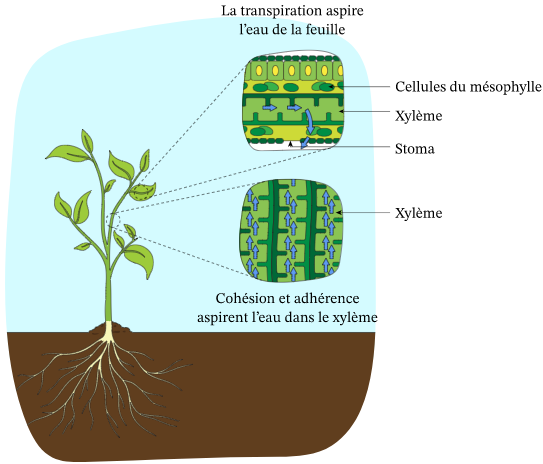
\includegraphics[width=\linewidth]{Image/waterflow_basics.png}
\captionof{figure}{Principe fondamental des flux hydriques dans les plantes \citep{nagwa_fiche_2023}.}
\label{fig:waterflow_basics}
\end{minipage}\hfill
\begin{minipage}{0.45\linewidth}
Comme illustré dans la figure \ref{fig:waterflow_basics}, la perte d'eau par transpiration au travers des stomates des feuilles augmente la tension dans le xylème. Cette tension se propage dans la plante par le principe de cohésion-tension jusque dans les racines.
Lorsque la tension est supérieure à celle du sol environnant, l'eau contenue dans la rhizosphère s'infiltre dans la racine et suit le gradient de potentiel hydrique par les chemins avec le moins de résistance.
Malgré les bonnes définitions des principaux mouvements et facteurs qui interviennent, les flux hydriques à l'échelle de la plante restent toutefois difficilement compréhensibles dans son ensemble \citep{lobet_plant_2014}.
\end{minipage} 
\newline

\noindent En effet, beaucoup de processus intervenant dans les flux hydriques ont pu être étudiés, compris et modélisés de façon précise.
Cependant, la manière dont tous ces processus interagissent avec le temps, l'espace et entre eux reste encore assez méconnue.
Ces différents processus sont aussi difficiles à mettre en relation du au fait qu'ils s'influencent les uns les autres et qu'ils peuvent, pour certains, être étudiés à des échelles très différentes.
\newline

Les flux hydriques peuvent être améliorés face aux sécheresses à l'aide de plusieurs processus.
La plante peut par exemple optimiser ses pertes en eau tout en conservant une activité suffisante (comme dans le cas de la fixation du carbone en C4).
Mais la plus grande marge d'adaptation pour faire face aux stress hydriques se situe sous le sol puisque c'est là que se déroulent les interactions sol-plante \citep{dunbabin_modelling_2013}. 
Il convient donc, spécialement dans le cadre de la résilience face à la sécheresse, de s'intéresser à l'absorption d'eau qui se déroule au niveau des racines. 

\subsection{Absorption d'eau}

L'absorption d'eau dans les racines est un phénomène clé pour comprendre les flux hydriques étant donné qu'il s'agit du point de départ de ces flux au sein de la plante.
Toutefois, cette partie du flux hydrique a longtemps été difficile à étudier dû à la difficulté que représente l'obtention des données racinaires puisqu'il est difficile d'y accéder de façon non destructrice.
Cependant, certaines innovations dans le domaine ont récemment permis l'acquisition de telles données de manière non destructrice (aéroponie, hydroponie, ...) permettant ainsi un plus grand accès aux données racinaires.
Ces nouvelles techniques offrent aujourd'hui la possibilité de quantifier certains points clés de l'absorption d'eau.
\newline

Quantifier avec précision les flux d'absorption d'eau depuis le sol dans les racines permettrait une meilleure compréhension de ceux-ci.
Mais cela requiert la prise en compte et la mise en relation d'une multitude de processus.
La figure \ref{fig:système sol-racine} reprend les trois grands composants, chacun étant caractérisé par plusieurs paramètres, qui constituent le système sol-racines : 

\begin{figure}[ht]
\centering
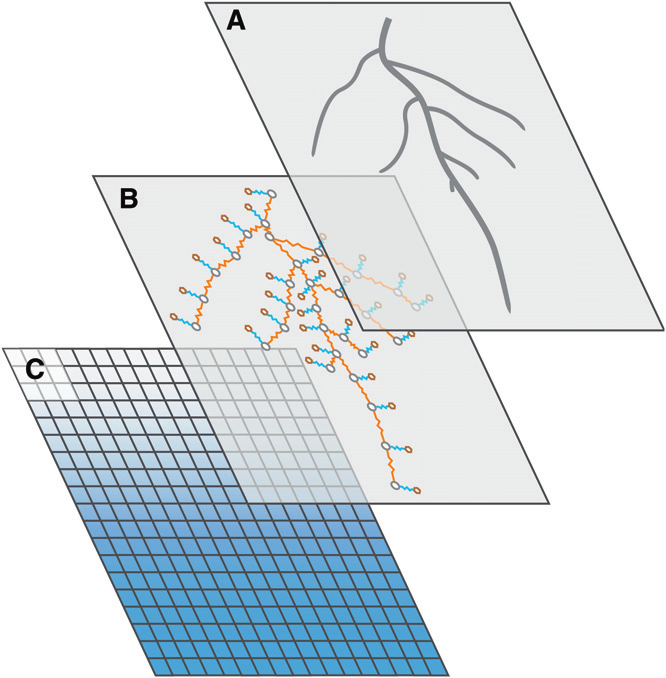
\includegraphics[width=0.5\textwidth]{Image/Properties of the soil root system.png}
\caption{Propriétés du système sol-racine \citep{lobet_plant_2014}}
\label{fig:système sol-racine}
\end{figure}

Ces trois composants sont :

\begin{itemize}
    \item A, l'architecture racinaire : le nombre de racines, leurs longueurs, leurs diamètres, leurs placements, ...
    \item B, l'architecture hydraulique de la racine : les résistances hydrauliques axiales $K_{x}$ (lignes oranges) et radiale $K_{r}$ (lignes bleues), de chaque segment racinaire (cercles gris) ainsi que des éléments du sol (cercles bruns).
    \item C, la distribution d'eau dans le sol.
\end{itemize}

Les caractéristiques du sol présentent donc déjà un grand intérêt.
Premièrement, elles définissent la réserve utile en eau du sol qui correspond à la quantité d’eau que le sol peut absorber et restituer à la plante.
Ensuite, la composition du sol influence le potentiel hydrique du sol et ainsi l'absorption d'eau par les racines.
Le sol définit donc la quantité d'eau disponible pour la plante. 
Ensuite, l'architecture racinaire définit la portée qu'a la plante pour explorer le sol et ainsi rendre accessible l'eau disponible dans le sol.
Finalement, l'anatomie racinaire, permet de quantifier l'entrée ($K_{r}$) et le transport ($K_{x}$) de l'eau jusqu'à la base de la tige.
\newline

La variabilité spatio-temporelle dans laquelle évolue une plante fait que des caractéristiques racinaires (architecturales et anatomiques) "parfaites" sont difficilement concevables.
Dès lors, il est préférable de partir du concept de système racinaire "adapté" à un environnement spécifique.
Les plantes ayant un phénotype plus adapté à la disponibilité des ressources dans l'espace et le temps auront un meilleur accès aux ressources comparé aux autres qui n'ont pas bénéficié de cette coïncidence \citep{lynch_steep_2013}.
Cette notion est formalisée sous le terme d'idéotype.

\subsection{Idéotype racinaire : steep, cheap and deep}

Un idéotype, pour une espèce agricole, est un modèle de plante qui correspond à un environnement donné et pas nécessairement à la plante idéale. 
Ce concept a été proposé par \cite{donald_breeding_1968} comme une nouvelle façon de concevoir la sélection végétale.
\newline 

Steep, cheap and deep (pentu, économe et profond) est un idéotype qui a été proposé pour optimiser la récupération d'eau et d'azote chez le maïs. 
Celui-ci décrit un phénotype avec des caractéristiques racinaires architecturales, anatomiques et physiologiques permettant une meilleure exploitation des couches de sols profondes.
L'idéotype est construit sur base du maïs car c'est, historiquement et encore à ce jour, une culture très répandue. 
Néanmoins, le maïs étant assez exigeant en eau et en azote, cet idéotype peut s'élargir à d'autres cultures ayant un système racinaire fondamentalement similaire (blé, riz, ...) et spécialement le sorgho qui a une architecture et une anatomie racinaire très semblable au maïs \citep{lynch_steep_2013}.
\newline

Steep, cheap and deep part de certains principes pour construire son système racinaire :

\begin{itemize}
    \item L'acquisition des ressources est fortement augmentée lorsque le placement des racines coïncide avec la présence de ressources dans le temps et l'espace.
    \item Le système racinaire représente un coût métabolique non négligeable \citep{kafkafi_respiratory_2002}. Plus le système racinaire est important, plus il est nécessaire de lui allouer des ressources.
    \item L'eau et l'azote sont plus facilement disponibles en profondeur durant la saison de croissance des plantes pour la plupart des sols.
    \item Les racines profondes ont plus de valeurs étant donné qu'elles participent également à l'absorption des ressources proches de la surface alors que les racines peu profondes n'ont pas la faculté d'explorer le sol en profondeur.
    \item L'utilité d'un trait racinaire est évaluée sur base de son coût métabolique et du bénéfice qu'il peut apporter.
\end{itemize}

La figure \ref{fig:steep, cheap and deep} ci-dessous reprend les traits racinaires de l'idéotype cheap, steep and deep dont les principaux seront développés par la suite.

\begin{figure}[ht]
\centering
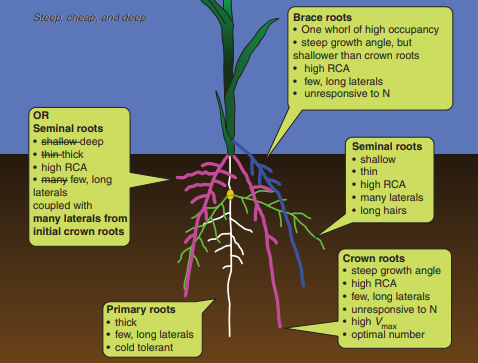
\includegraphics[width=0.75\textwidth]{Image/steep, cheap and deep.png}
\caption{L'idéotype steep, cheap and deep \citep{lynch_steep_2013}}
\label{fig:steep, cheap and deep}
\end{figure}

\subsubsection{Caractéristiques architecturales}

L'architecture du système racinaire (ASR) est une composante principale pour la productivité et la survie de la plante.
Celle-ci définit la quantité de ressources (eau et nutriments) qui est accessible par la plante dans un environnement dynamique et variable. 
L'ASR peut se caractériser par de multiples paramètres et de plus en plus de recherche sont faites afin d'identifier les paramètres clés qui contribuent à une meilleure résilience hydrique.
\newline

\noindent \textbf{La profondeur}

La profondeur est en fait le résultat d'autres paramètres de croissance tel que l'angle de croissance ou encore la vitesse de croissance primaire.
Les couches supérieures du sol sont les plus susceptibles de s'assécher lors d'un épisode de sécheresse. 
Cela est dû à l'évaporation et aux activités biologiques qui sont très importantes dans le haut de la rhizosphère.
Il est alors nécessaire que la plante soit capable de récupérer efficacement de l'eau dans les couches plus profondes du sol afin d'augmenter sa résistance en cas de sécheresse.
Lorsque la profondeur du sol le permet, augmenter la profondeur des racines améliore l'accès à l'eau.
Néanmoins, cette augmentation de la profondeur peut représenter un "gaspillage de photosynthèse" lorsqu'elle n'est pas accompagnée d'une densité de latérales suffisante dans les couches de sols profondes \citep{tardieu_any_2012}.
\newline

\noindent \textbf{La densité de latérale}

Les racines latérales développent considérablement la capacité de la plante à explorer le sol.
Néanmoins, trop de latérales demanderait un métabolisme trop important et réduirait la croissance de la racine mère \citep{lynch_root_2014}.
Plusieurs études ont montré que les coûts métaboliques de l'exploration du sol par les systèmes racinaires sont conséquents et peuvent dépasser 50\% de la photosynthèse quotidienne \citep{kafkafi_respiratory_2002}.
Il est dès lors favorable d'avoir moins mais de plus longues latérales capables d'explorer de plus grands volumes de sol tout en gardant un coût métabolique minimum.
Il serait également préférable que ces latérales soient uniformément distribuées le long de la racine primaire avec toutefois une densité plus élevée dans les couches moyenne et profonde du sol pour améliorer l'absorption en profondeur \citep{wasson_traits_2012}.
\newline

\noindent \textbf{Diamètre}

Un diamètre plus large permet une meilleure pénétration lorsque le sol est dur \citep{bengough_root_2011}.
De plus, il a été observer qu'un diamètre plus large de la racine primaire est lié à un plus grand potentiel de croissance \citep{pages_estimating_2010}.
Une racine ayant un plus grand diamètre est ainsi plus disposée à atteindre les couches plus profondes du sol.
\newline

\noindent \textbf{Tropisme}

En adaptant son système racinaire en fonction de ces stimuli environnementaux, la plante maximise son accès aux ressources et cela participe à augmenter sa résilience dans le cas ou la présence d'eau ou nutriments est limitée.
Les plantes réagissent différemment à ces stimuli et cette capacité d'adaptation peut représenter un atout en condition de manque de ressources.
Il a entre autre été observé par \cite{gul_hydrotropism_2023} que différentes espèces/variétés peuvent avoir un hydrotropisme plus ou moins important illustrant ces différences d'adaptation entre plants.

\subsubsection{Caractéristiques anatomiques}

L'anatomie racinaire impacte l'entrée des ressources dans la plante et l'efficacité avec laquelle elles sont allouées en son sein.
Il est donc intéressant de s'y attarder pour modifier l'architecture hydraulique des racines et ainsi améliorer la résistance au stress.
Un segment racinaire se différencie par sa conduction hydraulique axiale et radiale ainsi que la conductance du chemin le plus court qui le relie à la base de la tige \citep{lobet_plant_2014}.
\citep{wasson_traits_2012} avancent que de plus grandes conductivités axiale et radiale augmentent la capacité de la plante à récupérer et à transporter l'eau contenue dans les sols profonds. 
\newline

\noindent \textbf{Conductivité radiale}

La conductivité radiale permet l'entrée d'eau depuis le sol dans les racines.
Celle-ci est largement influencée par la succession de couches qu'il peut y avoir entre la surface de la racine et le xylème.

\begin{minipage}{0.55\linewidth}
\captionsetup{type=figure,hypcap=true}
\centering
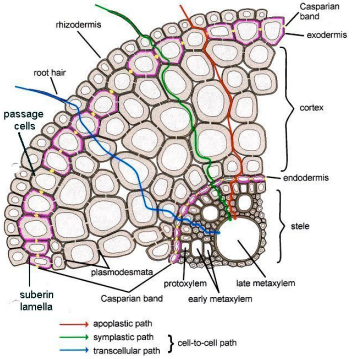
\includegraphics[width=\linewidth]{Image/radial flow.png}
\captionof{figure}{Conductivité radiale \citep{ranathunge_new_2005}.}
\label{fig:radial flow}
\end{minipage}\hfill
\begin{minipage}{0.4\linewidth}
La figure \ref{fig:radial flow} illustre les différentes voies par lesquelles l'eau peut s'infiltrer jusqu'au xylème ainsi que les différentes couches qui composent ces chemins.
La conductivité radiale est largement influencée par la succession de couches, leurs anatomies ainsi que la présence de cadres de Caspary qui sont des structures hydrophobes \citep{yang_drought-induced_2012}.
L'anatomie racinaire est altérée à long terme par les conditions environnementales.
Les structures hydrophobes peuvent, par exemple, être mises en place suite à un épisode de sécheresse \citep{vandeleur_role_2009}.
À court terme, la plante peut également s'adapter aux conditions dans la rhizosphère via la régulation des aquaporines qui peuvent, pour certaines espèces, participer jusqu'à 80\% du flux radial \citep{javot_role_2003}.
\end{minipage} 
\newline

\noindent \textbf{Conductivité axiale}

La conductivité axiale mesure le déplacement de la sève minérale au sein de la plante.
Celle-ci peut, comme la conductivité radiale, être altérée par des mécanismes qui l'influence à long et court terme.
Parmi les caractéristiques qui impactent sur le long terme, on retrouve : la taille, le nombre et la qualité d'interconnexions des vaisseaux de xylème qui sont les conduits du flux axial.
En ce qui concerne l'influence à court terme de la conductivité axiale, les principaux phénomènes sont les embolies causées par des cavitations dans les vaisseaux de xylèmes.
La cavitation intervient lorsque la tension créée dans le xylème par la transpiration des feuilles devient trop importante.
Il se crée alors des bulles de gaz dans le xylème, ce qui rend les vaisseaux concernés hermétiques au passage de l'eau, ce qui limite ainsi les flux d'eau aux autres vaisseaux qui n'ont pas de cavités.
Il a été montré par \cite{delzon_mechanism_2010} que la susceptibilité à la cavitation est liée à la taille des vaisseaux de xylème, à la rugosité des parois et à l'abondance de perforation dans le xylème.
Optimiser ces caractéristiques peut donc participer à réduire les phénomènes de cavitation dans les plantes.
\newline

\noindent \textbf{Root Cortical Aerenchyma (RCA)}

L'aérenchyme est un tissu végétal constitué de cellules séparées par de grandes cavités.
Son intérêt dans les racines a longtemps été réduit à faciliter des transferts gazeux lorsque les plantes font face à l'hypoxie.
Cependant, il est aujourd'hui également considéré que sa présence permet une meilleure exploration des sols par les racines en réduisant leurs coûts métaboliques.
Le RCA réduit les besoins en respirations et en nutriments des tissus racinaires, ce qui permet une plus grande croissance racinaire pour un même coût métabolique.
Sa présence est donc favorable dans des conditions déficitaires en eau bien que l'aérenchyme peut réduire le flux d'eau radiale dans les racines.


\subsubsection{Caractéristiques physiologiques}

La physiologie des plantes joue un rôle crucial dans la capacité des plantes à survivre et à s'adapter à leur environnement.
Les plantes sont capables de s'adapter à leur environnement en réagissant aux stimuli externes qu'elles reçoivent.
La morphologie des poils racinaires, les exsudats racinaires, une augmentation de la croissance racinaire ou encore les différents tropismes sont des mécanismes dont dispose la plante pour modifier son ASR et ainsi répondre aux conditions environnantes \citep{dunbabin_modelling_2013}.
L'architecture et l'anatomie racinaire de la plante découlent donc en partie de la physiologie de la plante.
\newline

Le "root cost of acquisition", qui est plus une conséquence de l'anatomie, l'architecture et la physiologie, mesure essentiellement l'habileté de la plante à acquérir des ressources en fonction de l'investissement mis dans la production de ses racines.
Dans cet idéotype, l'idée est de minimiser le coût énergétique et matériel pour produire les racines tout en maximisant leur disposition à explorer le sol en profondeur et à extraire l'eau nécessaire à la plante.
La présence d'aérenchymes peut, par exemple, améliorer le "coût d'acquisition de ressources" en réduisant le coût métabolique des racines.
De même que la présence de longue latérale bien répartie.
\newline

\subsection{Modélisation des flux hydriques dans les racines}

Modéliser les flux hydriques dans le système sol-plante nécessite l'intervention d'une multitude d'éléments.
Ces éléments sont, pour beaucoup, dynamiques et hétérogènes, ce qui complique l'appréhension du système dans sa globalité.
\cite{passot_connecting_2018} imaginent un réseau qui représente les outils, propriétés et variables d'états nécessaires pour quantifier les interactions entre les différents éléments du système sol-plante.
Ce réseau fait intervenir des procédures expérimentales, des outils informatiques et des données propres aux flux hydriques.
La figure \ref{fig:modelling} représente la partie considérée dans ce travail de ce réseau (le réseau complet est disponible en annexe \ref{an:modelling_full}).
Le réseau réduit est alors compartimenté en fonction de deux "dimensions" et de deux "échelles".
Les flux hydriques peuvent être caractérisés à l'échelle d'un organe ou de la plante.
De plus, il serait également nécessaire de prendre en compte des aspects structurels et fonctionnels.
\newpage

\begin{figure}[ht]
\centering
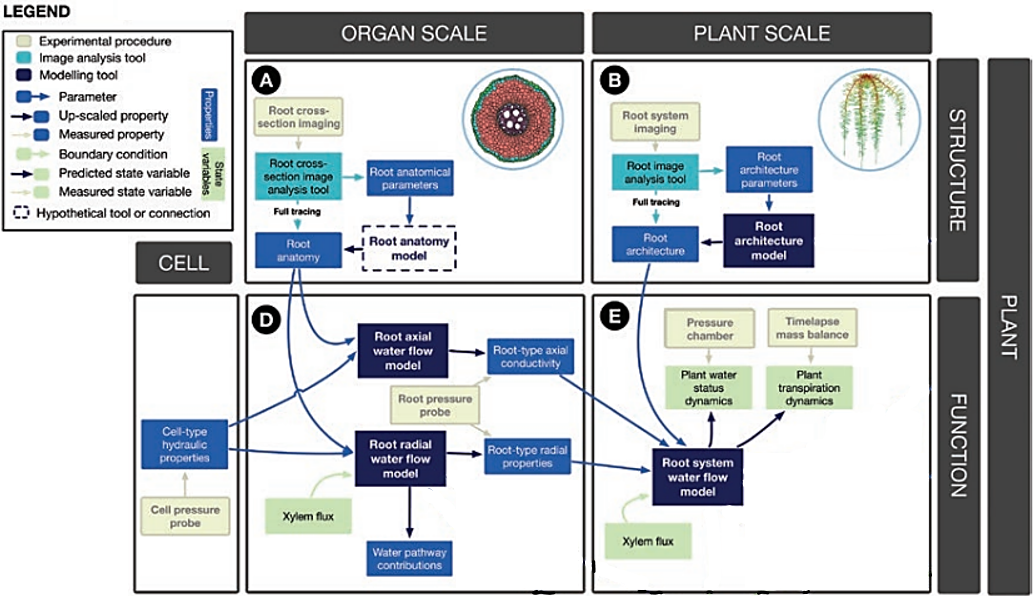
\includegraphics[width=1\textwidth]{Image/modelling_b.png}
\caption{Quantifier les relations hydriques dans le système sol-plante. Réseaux réduit de \cite{passot_connecting_2018}}
\label{fig:modelling}
\end{figure}

\subsubsection{Échantillonnage}
\textbf{Architecture}
\newline
Un problème persistant pour modéliser l'architecture racinaire est l'acquisition de données.
Les données en champs représentent la réalité, mais elles demandent beaucoup de travail et il est difficile d'isoler l'impact d'un facteur précis.
Il est alors nécessaire de procéder en laboratoire ou à l'aide de caractères "proxy" en champs pour quantifier certains traits racinaires spécifiques \citep{wasson_traits_2012}.
Un "proxy" est une mesure racinaire ou aérienne qui serait une conséquence ou du moins corrélée avec le phénotype étudié (exemple : la croissance primaire serait un proxy pour calculer la profondeur de la racine).
\newline

Bien entendu, ces deux méthodes créées un biais dans les données récoltées.
Les expériences en laboratoire permettent d'isoler un facteur en particulier, ce qui permet une étude plus fine de ce facteur.
Mais cela se fait au détriment du réalisme dans lequel se développe le système racinaire.
Les effets de compétitions ou les associations entre organismes sont ignorés, de même que le contenant, le substrat, les nutriments sont définis par l'étude réalisée.
De l'autre côté, l'utilisation d'un proxy sur des données "réalistes" en champs suppose une relation parfaite entre la mesure qui est effectuée et le trait architectural d'intérêt trop difficile à mesurer.
\newline

\textbf{Anatomie}
\newline
L'observation d'échantillon pour l'anatomie racinaire présente plus de facilité que pour l'architecture.
En effet, une section racinaire transversale au microscope permet une vue globale de l'anatomie racinaire d'une racine.
Il n'est alors, dans la majorité des cas, pas trop difficile de parvenir à voir clairement l'ensemble de l'anatomie sans avoir à faire trop de manipulations comme cela peut être le cas pour l'architecture.
Un autre avantage est qu'il n'est pas nécessaire d'observer l'anatomie au cours du temps, un échantillon de fin de culture suffit souvent dans le cas de l'anatomie.

\subsubsection{Modélisation structurelle}

La structure d'un système racinaire peut être décrite à l'échelle de l'organe, ce qui correspond à l'anatomie racinaire, ou à l'échelle de la plante qui correspond alors à l'architecture racinaire.
Dans chacun de ces deux cas, cette structure peut être retracée entièrement sur base d'une observation directe.
Cette méthode s'appelle le "full tracing" et demande énormément de travail, de temps et de rigueur.
Cette méthode présente une alternative qui est la modélisation.
Il suffit alors de tracer une partie de l'anatomie/architecture et d'en extraire des paramètres qui permettent par la suite de reformer, aussi fidèlement que possible, l'ensemble de l'organe ou de la plante.
Chaque modèle se base sur un nombre limité de paramètres requis en input qui sont ainsi considérés comme plus représentatifs d'une architecture/anatomie racinaire.
Les autres caractéristiques sont dans ce cas stochastiques ou construites sur base des inputs.
L'utilisation de tel ou tel modèle demande donc de sélectionner les inputs qui seront considérés.
Cela permet finalement de générer bon nombre d'architectures de systèmes racinaires parfois très contrastés les unes des autres.
\newline

La figure \ref{fig:structure generation}, qui condense la partie structurelle du réseau précédemment présenté (figure \ref{fig:modelling}), illustre la démarche globale permettant la génération de structures racinaires (anatomique ou architecturale).

\begin{figure}[ht]
\centering
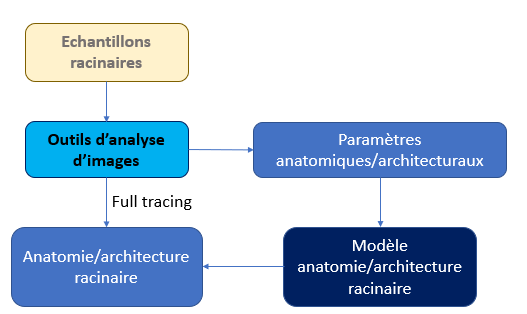
\includegraphics[width=0.5\textwidth]{Image/structure generation.png}
\caption{Génération d'une structure (anatomie ou architecture) de système racinaire}.
\label{fig:structure generation}
\end{figure}

Les données récoltées (de publication préexistante ou d'échantillons racinaire) permettent de mesurer/quantifier des caractéristiques racinaires.
Les caractéristiques considérées comme étant plus déterminantes sont extraites et introduites dans un modèle qui va recréer l'ASR ou l'anatomie sur base de ces quelques caractéristiques.
Finalement, l'architecture/anatomie générée par le modèle devrait correspondre à ce que l'on aurait pu observer empiriquement via le "full tracing" mais qui aurait demandé énormément de rigueur et de travail afin de tout mesurer.

\subsubsection{Modélisation fonctionnelle}

La modélisation fonctionnelle utilise les structures préalablement construites pour quantifier les différents processus de flux hydriques.
Le flux radial ainsi que le flux axial dépendent en partie de l'anatomie racinaire.
Il est donc possible, sur base de celle-ci ainsi que certaines propriétés hydriques (e.g. équation de Hagen-Poiseuille) et modèles (e.g. MECHA), d'estimer le flux radial et le flux axial au niveau d'un segment racinaire.
\newline

Finalement, en récupérant la conductivité axiale ainsi que les propriétés du flux radial, il est possible d'intégrer ces flux à l'ensemble de l'architecture racinaire et ainsi obtenir un modèle pour les flux hydriques dans le système racinaire (e.g.MARSHAL).

\subsection{Le sorgho}
Le sorgho est une monocotylédone de la famille des Poaceae qui est cultivée entre mai et octobre.
C'est une plante herbacée annuelle qui peut être cultivée pour ses grains (sorgho grains) ou comme fourrage (sorgho fourrager).
Le sorgho figure, selon la FAO ( l'Organisation des Nations unies pour l'alimentation et l'agriculture), parmi les céréales les plus cultivées dans le monde. 
Celui-ci est à ce jour principalement répandu en Afrique, Asie et Amérique du Sud en raison de sa bonne acclimatation aux climats chauds et arides.
Ses multiples intérêts : alimentation humaine, alimentation animale (fourrage et grain) et application industrielle (agro-carburant, ...) confère au sorgho une certaine importance et sa résilience hydrique pourrait le rendre incontournable au vu des changements climatiques observés.
\newline

En effet, le sorgho est connu pour avoir une grande tolérance face à la sécheresse. Plusieurs causes ont déjà été identifiées pour tenter de comprendre cette résilience telle que :
\begin{itemize}
    \item Fixation du carbone en C4 qui permet de limiter les pertes d'eau par l'ouverture des stomates nécessaire pour la photosynthèse. Les plantes en C4 ont ainsi une meilleure efficience photosynthétique et sont plus adaptées aux climats chaud et sec \citep{shanker_c4_2011}.
    \item Un rapport $\frac{racines}{pousses}$ qui augmente lorsqu'il y a une diminution de l'humidité du sol, ce qui représente un mécanisme de survie face à la sécheresse \citep{mwamahonje_drought_2021}.
    \item L'aptitude "Stay-green" qui représente une bonne adaptation à la sécheresse.
    Celui-ci consiste pour la plante à réduire la taille du couvert à la floraison, ce qui permet d'assurer une disponibilité en eau suffisante pendant le remplissage des grains et ainsi de meilleurs rendements en cas de sécheresse.
    \item Un système racinaire réputé assez profond et étendu.
\end{itemize}
Le sorgho est donc une culture idéale dans les régions où l'eau et les nutriments sont limités. 
En étudiant le système racinaire du sorgho, il serait intéressant de comprendre comment les racines de cette plante participent à la résilience hydrique de la plante.
\newline

Le système racinaire du sorgho est déjà caractérisé de "robuste" et participerait effectivement à faire face aux conditions environnementales difficiles, notamment la pénurie d'eau.
Le schéma \ref{fig:RSA} illustre l'organisation classique du système racinaire des Graminées comme le sorgho.

\begin{figure}[ht]
\centering
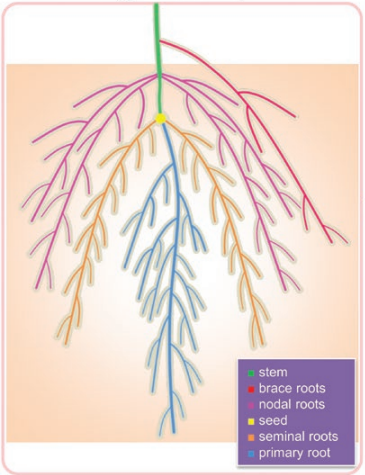
\includegraphics[width=0.5\textwidth]{Image/RSA.png}
\caption{Illustration d'un système racinaire de Graminée \citep{correa_soil_2019}}.
\label{fig:RSA}
\end{figure}

Au début de la germination, le sorgho développe une seule racine primaire qui produit de nombreuses ramifications secondaires.
Le sorgho, contrairement au maïs, ne développe pas de racine séminale en plus de la racine primaire.
Les racines nodales se forment ensuite successivement, prenant la place de la racine séminale qui disparaît progressivement.
Les nœuds souterrains produisent une quantité croissante de racines nodales en fonction de leur position.
Lorsque les racines nodales se développent à partir des nœuds aériens, leur insertion est nettement verticillée \citep{kumar_goyal_how_2021}.
\newline

Plusieurs acteurs de l'agriculture en Belgique s'intéressent depuis quelques années à une potentielle implantation du sorgho dans les régions aux climats tempérés comme en Belgique.
On retrouve, entre autre, le Centre Indépendant de Promotion Fourragère (CIPF).
Le CIPF expérimente et vulgarise différents sujets liés aux cultures de maïs, miscanthus, silphie ou encore le sorgho.
Ainsi, depuis 2013, le CIPF réalise différents tests culturaux sur le sorgho afin d'étudier l'intérêt agronomique que peuvent avoir les différentes variétés.
Il partage ensuite les résultats obtenus dans le but de conseiller/déconseiller une culture de sorgho.
\newpage

\section{Objectifs}

Le sorgho, depuis longtemps cultivé dans les régions tropicales semi-arides d'Afrique et d'Asie, est une culture que l'on pourrait voir s'étendre dans des régions plus au nord.
Cet intérêt particulier qui lui est voué provient du fait que le sorgho offre les mêmes débouchés que le maïs qui figure parmi les plus grandes cultures dans le monde.
Il serait imaginable que le sorgho, après avoir bénéficié de recherche et sélection, monte au classement des céréales les plus cultivées dont il occupe déjà la cinquième place.
\newline

Le sorgho, en plus d'offrir une multitude de services, possède un atout qui intéresse le monde agricole actuellement : son impressionnante résistante à la sécheresse.
Plusieurs mécanismes morphologiques et physiologiques participant à cette résilience hydrique ont déjà été identifiés.
Toutefois, plusieurs pistes situées dans le système racinaire restent à ce jour inexplorées.
Il est connu et prouvé que le sorgho possède un système racinaire assez profond et étendu grâce à ses nombreuses racines nodales.
Cependant, le développement de l'architecture racinaire ainsi que l'impact qu'a celle-ci sur l'extraction d'eau du sol sont à ce jour peu étudié.
\newline

Ce mémoire s'inscrit dans cette démarche et s'intéresse donc à la modélisation du système racinaire de sorgho afin d'en identifier les traits particuliers.
Les objectifs sont alors :
\begin{enumerate}
    \item Caractériser et quantifier le système racinaire de six variétés de sorgho testées au CIPF. 
    \item Identifier les potentielles différences entre ces variétés.
    \item Modéliser l'architecture du système racinaire du sorgho.
    \item Comparer les modélisations de systèmes de sorgho à ceux du maïs (similaire mais moins tolérant au stress hydrique).
\end{enumerate}

Plus globalement, ce travail s'inscrit dans une étude qui vise à comprendre les flux hydriques au sein des plantes.
Dans l'optique, nécessaire à ce jour, de sélection variétale et génétique de culture plus résilientes aux fréquentes sécheresses, le sorgho a aujourd'hui une avance confortable.
Comprendre comment le système racinaire du sorgho participe à lui offrir une meilleure tolérance aux stress hydriques que le maïs offre des pistes pour la sélection des variétés d'une multitude d'autres espèces face aux changements climatiques.
Néanmoins, ce travail est loin d'être exhaustif et ne peut, à son échelle, qu'apporter une pierre à l'édifice du travail de recherche bien large sur les flux hydriques au sein des plantes. 
Comme mentionné précédemment, la modélisation de système racinaire seule n'a que peu de valeur.
C'est en incluant cela dans un réseau (comme présentée en figure \ref{fig:modelling}) qu'il est alors possible d'améliorer la compréhension globale des flux hydriques au sein du système sol-plante.
\newpage

\section{Méthodologie}

\subsection{Sélection des génotypes}
Afin d'élargir la portée des expériences, il a été décidé de travailler sur plusieurs variétés.
Les génotypes ont été sélectionnés sur base des variétés testées précédemment par le centre indépendant de promotion fourragère (CIPF).
Les six variétés échantillonnées correspondent à celles qui ont été testées, au minimum l'année précédente et l'année en cours (à savoir 2021 et 2022).
Ce choix confère plusieurs avantages :
\begin{itemize}
    \item Premièrement, les résultats des précédentes cultures réalisées et analysées par le CIPF offrent des informations sur les parties aériennes des six variétés considérées sur au moins deux années consécutives.
    \item Ensuite, les cultures de 2022 ayant été récoltées en septembre, il a été possible de récupérer des échantillons racinaires de cette culture, offrant ainsi des échantillons de fin de culture.
\end{itemize}
Ces six génotypes étudiés sont repris dans le tableau \ref{tab:variete} ci-dessous ainsi que l'identifiant attribué à ces génotypes qui sera par la suite utilisé pour différencier les échantillons.

\begin{table}[ht]
    \centering
    \caption{Génotypes}
    \begin{tabular}{c c c}
        \hline
        \textbf{Identifiant} & \textbf{Variété} & \textbf{Type} \\
        \hline
        \hline
        A & Amiggo & Sorgho fourrager monocoupe \\
        B & RGT Biggben & Sorgho fourrager monocoupe \\
        H & ES Hyperion & Sorgho fourrager monocoupe \\
        J & KWS Juno & Sorgho fourrager monocoupe \\
        S & RGT Swingg & Sorgho fourrager monocoupe \\
        V & Vegga & Sorgho fourrager monocoupe
    \end{tabular}
    \label{tab:variete}
\end{table}

\subsection{Parties aériennes}
Les données des parties aériennes proviennent des rapports d'expériences partagés par le CIPF \citep{cipf_resultats_2021,cipf_resultats_2022}.
Ces rapports reprennent plusieurs informations :
\begin{itemize}
    \item Protocole expérimental : densité de semis, date de culture, culture précédente, fumure, traitement des semences, ...
    \item Des données météorologiques : pluviométrie, température, ...
    \item Les résultats de culture : \% de masse sèche (MS), rendement MS, \% de levée, hauteur des plants, valeur alimentaire, ...
\end{itemize}
Certains résultats de ces rapports ont été récupérés et rassembler dans un document Excel pour permettre leur utilisation dans R.

\subsection{Échantillons racinaires}

Les dates de culture de sorgho ainsi que les difficultés expérimentales décrites précédemment ont rendu nécessaire l'obtention d'échantillon de différentes façons.
D'une part, des échantillons racinaires de fin de culture ont été récoltés suite aux tests de cultures réalisés par le CIPF. 
Il s'agit donc de plants de sorgho ayant été cultivé du 17 mai au 21 septembre 2022 et en champ.
D'autre part, des résultats de début de culture sont récupérés via une expérience réalisée en serre et sur une période bien plus courte d'une vingtaine de jour (du 3 avril au 24 avril 2023).
Tous les échantillons racinaires ont été numériser à l'aide du scanner Epson Perfection V850 Pro.
Les scans ont été faits avec la configuration disponible en annexe \ref{an:config}.

\subsubsection{Fin de culture CIPF}

\begin{minipage}{0.4\linewidth}
\captionsetup{type=figure,hypcap=true}
\centering
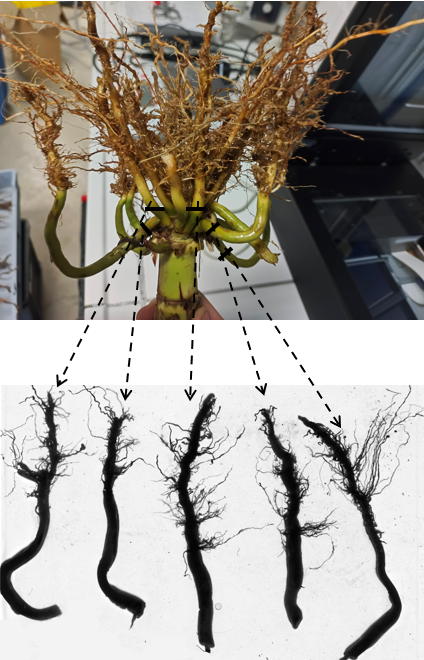
\includegraphics[width=0.65\linewidth]{Image/scan.png}
\captionof{figure}{Numérisation échantillons racinaires}
\label{fig:scan}
\end{minipage}\hfill
\begin{minipage}{0.5\linewidth}
Les données de fin de culture sont récupérées sur des échantillons racinaires résultant des tests réalisés par le CIPF.
Un résumé du protocole de culture respecté par le CIPF lors de leurs tests de culture de sorgho est disponible en annexe \ref{an:protocole_CIPF}.
Suite à la récolte des parties aériennes, quatre systèmes racinaires de plants de sorgho ont été récupérés de façon aléatoire à la bêche en champ pour chacune des six variétés étudiées.
Les 24 systèmes racinaires ont ensuite été conservés dans le bloc de terre extrait en chambre froide jusqu'à ce qu'ils soient nettoyés et numérisés.
Afin de pouvoir scanner ces échantillons, les racines ont été coupées pour permettre de les scanner en plusieurs parties.
L'image \ref{fig:scan} montre un des systèmes racinaires nettoyés ainsi que le résultat de la numérisation d'une partie de celui-ci.
\end{minipage} 
\newline

\subsubsection{Début de culture UCLouvain}
Les racines de plants de début de culture ont été échantillonnés à l'aide de rhizotrons dans les serres de l'UCLouvain.
\newline

\textbf{Rhizotron} \\
Un rhizotron est un montage permettant d'observer le développement racinaire ainsi que la prise de mesure précise de l'architecture racinaire de façon non destructrice.
Pratiquement, les rhizotrons ont été construits comme illustré par la figure \ref{fig:rhizotron}.
Une planche en bois sur laquelle se trouve des mousses est remplie d'un substrat au choix.
Une feuille de papier filtre laissant passer la solution nutritive est ensuite placée sur le substrat.
Finalement, une plaque de plexiglas vient fermer le dispositif avec la graine placée entre le papier filtre et la plaque transparente.
La racine est ainsi visible et peut accéder aux nutriments apportés par l'arrosage du substrat à travers le papier filtre.
\newpage

\begin{figure}[ht]
\centering
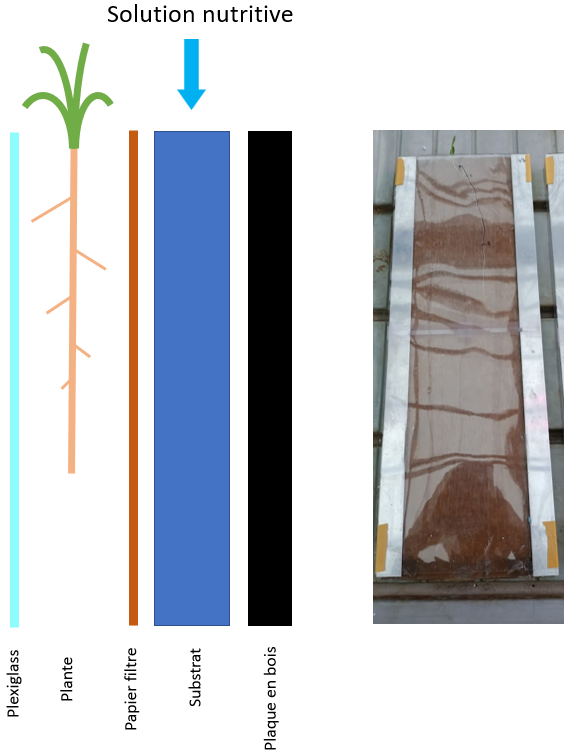
\includegraphics[width=0.5\textwidth]{Image/rhizotron.png}
\caption{Montage rhizotron}
\label{fig:rhizotron}
\end{figure}

Quatre rhizotrons de dimension 60×20 cm ont été réalisés pour chacune des six variétés étudiées faisant un total de 24 rhizotrons contenant chacun un plant de sorgho.
Ceux-ci ont été placés dans la serre 'S.0 27' à l'UCLouvain qui simule un climat tempéré.
Les rhizotrons sont entreposés par six dans des bacs comme montrés en figure \ref{fig:montage}.
Des bouts de polystyrène sont posés au fond des bacs pour permettre l'évacuation de la solution nutritive non absorbée par les racines et empêcher que le bois ne beigne dedans.
La partie du rhizotron laissant apercevoir le système racinaire a systématiquement été placé derrière un autre rhizotron ou derrière une planche pour ceux de devant afin d'éviter une intervention de phototropisme sur les racines.
De plus, les rhizotrons ont été inclinés avec un angle d'environ 30° dans le but de favoriser la croissance de la racine entre le plexiglas et le papier filtre pour que celle-ci reste visible.
\newpage

\begin{figure}[ht]
\centering
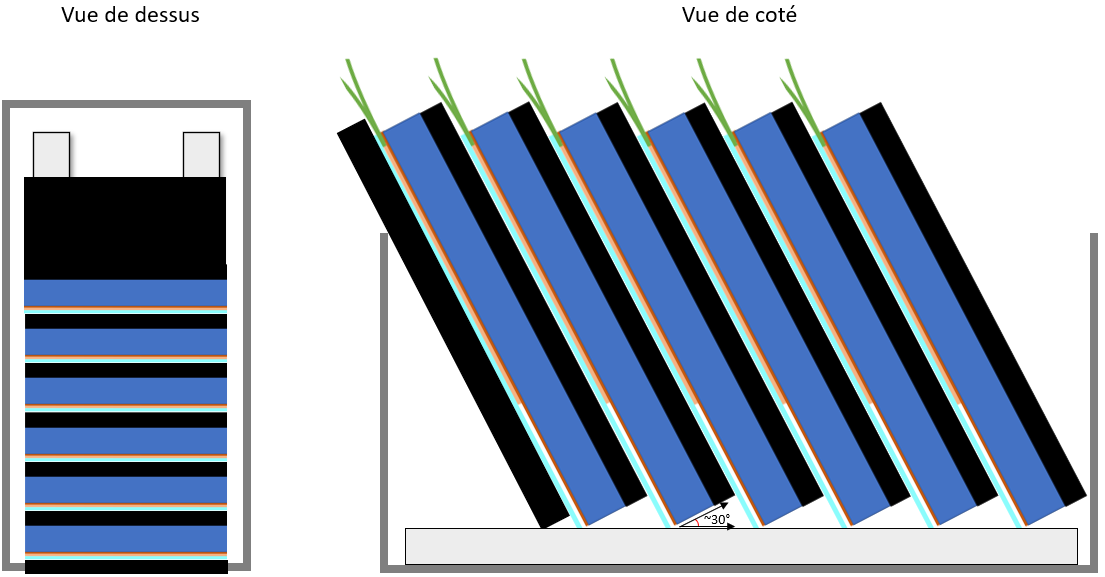
\includegraphics[width=0.75\textwidth]{Image/montage.png}
\caption{Expérience}
\label{fig:montage}
\end{figure}

Le substrat qui est utilisé est de la perlite.
Il s'agit d'un substrat de culture léger, avec une bonne rétention d'eau, ce qui peut favoriser une croissance saine des racines et des plantes.
Chaque rhizotron a été arrosé les lundi, mercredi et vendredi durant toute la durée de l'expérience avec 50 ml de solution de Hoagland.
La solution de Hoagland, dont la composition est reprise en annexe \ref{an:Hoagland}, contient tous les nutriments nécessaires au développement de la majorité des plantes.
Cette fréquence d'arrosage vise à apporter une quantité suffisante d'eau et de nutriment pour permettre aux plantes de se développer sans être exposées à l'un ou l'autre stress.
Un tracé de l'évolution des racines a été effectué de façon régulière afin de pouvoir mesurer des paramètres de croissance.
L'un de ces tracés est disponible en annexe \ref{an:trace}.
\newline

Une première salve de rhizotron s'est avérée être inutilisable dû à la présence de pathogènes dans le dispositif expérimental.
Ceux-ci ont été identifier comme étant des champignons (Stachybotrys echinata et Stachybotrys chartarum).
Une seconde salve a donc été réalisée avec des précautions supplémentaires.
Les échantillons utilisés dans ce travail ont, en conséquence, été traités avec un fongicide (Rovral) une première fois avant le montage des rhizotrons et deux fois supplémentaires au cours de la croissance des plants.
Bien que cela a partiellement réduit l'apparition de champignons, ceux-ci ont malgré tout été observés dans les rhizotrons utilisés et peuvent de ce fait avoir influencé la croissance des plants.

\subsection{Numérisation des échantillons}
L'acquisition des échantillons précédemment décrite permet de quantifier certaines caractéristiques de l'architecture racinaire chez ces six variétés de sorgho.
Certains problèmes évoqués auparavant se présentent pour les deux sets d'échantillons (fin de culture en champs et début de culture en rhizotron).
Les systèmes racinaires en champs sont ceux de plantes ayant terminé leurs croissances et sont alors très importants.
Cela rend les mesures complexes à réaliser car les racines sont assez longues et se chevauchent.
Les racines provenant des rhizotrons permettent quant à elles des mesures précises et temporelles, mais résultent de conditions assez artificielles et ne donnent pas l'état final des racines.
De ce fait, la quantification se fera, compte tenu du paramètre mesuré, sur des échantillons de fin de culture ou de début de culture.

\subsubsection{Smartroot}

\begin{minipage}{0.5\linewidth}
\captionsetup{type=figure,hypcap=true}
\centering
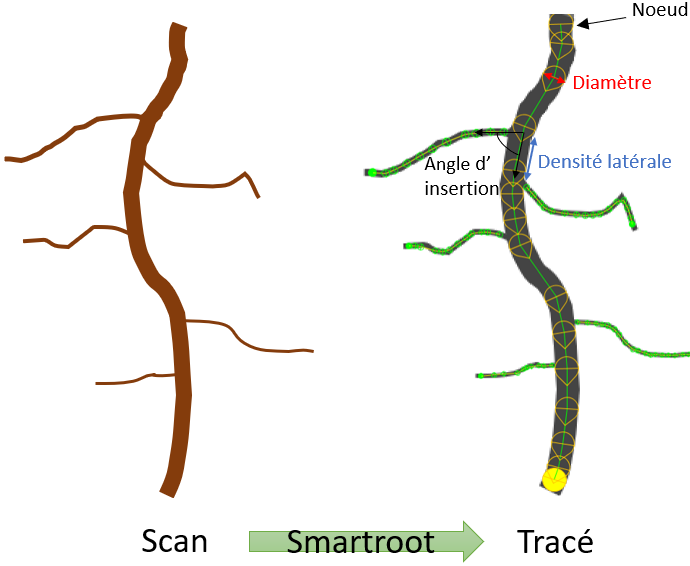
\includegraphics[width=1\linewidth]{Image/schema smartroot.png}
\captionof{figure}{Smartroot}
\label{fig:schema smartroot}
\end{minipage}\hfill
\begin{minipage}{0.45\linewidth}
Toutes les mesures réalisées sur les échantillons racinaires ont été faites à l'aide de Smartroot \citep{lobet_novel_2011}.
Smartroot est un logiciel d'analyse d'images basé sur ImageJ qui permet la quantification de la croissance et d'architecture racinaire complexe.
Cette quantification se fait via le traçage d'image d'échantillon de système racinaire (figure \ref{fig:schema smartroot}).
Les racines sont représentées par un ensemble de points (appelés nœuds) reliés entre eux.
Le logiciel est par la suite capable, sur base des nœuds de fournir des mesures de l'architecture du système racinaire tel que la longueur, le diamètre, la densité de latérale, l'angle d'insertion des latérales, ...
\end{minipage} 
\newline

\noindent Les logiciels d'analyse d'image peuvent être classé en trois catégories :
\begin{itemize}
    \item Manuel : Qui ont l'avantage de pouvoir être utilisable dans presque toutes les situations, mais qui requièrent énormément d'interactions et donc de travail pour l'utilisateur.
    \item Automatique : Qui ne fonctionnement souvent que dans des cas très spécifiques adaptés au logiciel, mais qui sont très rapides et demande peu de travail.
    \item Semi-automatique : Qui utilisent des algorithmes permettant de faciliter et d'accélérer l'analyse d'image à l'aide d'interventions de la part de l'utilisateur pour corriger/orienter les algorithmes.
\end{itemize}
Smartroot a été conçu pour réaliser les tracés racinaires de façon semi-automatique.
Cela permet de considérablement réduire le temps et le nombre d'interactions nécessaires de l'utilisateur tout en restant modulable à bon nombre de situations.

\subsubsection{Structure des données}

Le fichier qui contient le tracé des racines est enregistré en utilisant le format Root System Markup Language (RSML) \citep{lobet_plant_2014}.
Ce format est essentiellement un fichier XML (eXtensible Markup Language) qui contient des informations topologiques, géométriques et autres données numériques qui permettent de capturer la complexité d'un système racinaire (en 2D, 3D et données temporelles).
Le langage XML est largement utilisé pour échanger des données entre des applications hétérogènes, car il est facile à lire et à écrire pour les humains et les machines. 
Il est également extensible, ce qui signifie que les développeurs peuvent définir leurs propres balises pour représenter des données spécifiques à leur application (dans le cas du RSML, des données racinaires).
Une représentation visuelle de la structure d'un fichier RSML est disponible en annexe \ref{an:RSML}.
Smartroot propose par ailleurs la possibilité d'extraire directement les données racinaires plus globales dans un fichier CSV (Comma separated values).
Ce fichier contient alors entre autres la longueur, le diamètre moyen, l'angle d'insertion, la direction de chaque racine.
Les analyses descriptives ainsi que l'inférence statistique seront dès lors réalisés sur base de ces fichiers.
\newline

Tous les fichiers de données RSML et CSV résultants de la numérisation des échantillons et de l'utilisation de Smartroot sont disponibles sur \href{https://github.com/ndegives/Memoire}{Github}.
Les échantillons suivent les nomenclatures suivantes :
\begin{itemize}
    \item Parties aériennes : Les données moyennes sont simplement organisées à l'aide du nom de la variété.
    \item Les échantillons de fin de culture : Chaque racine est nommée comme suit :
    \begin{center} Identifiant variété\_Numéro de plante\_N\oe ud de la racine\_ Racine (e.g. A2\_1\_4) \end{center}
    \item Les échantillons en rhizotron : Chaque plant est identifié par l'identifiant de la variété suivi d'un numéro pour identifier le plant au sein de la variété (e.g. S2)
\end{itemize}

\subsection{Modélisation de l'architecture racinaire}

Suite à l'analyse des images provenant des différents échantillons racinaire, il est possible de travailler avec les données chiffrées qui en résultent.
Dans un premier temps, une caractérisation sera faite afin d'identifier les valeurs de certain paramètre d'architecture racinaire propres au sorgho.
Ensuite, des paramètres seront introduits en input d'un modèle afin de reconstruire un système racinaire complet.

\subsubsection{ArchiSimple}

ArchiSimple  \citep{pages_calibration_2014} est un modèle permettant la génération d'ASR.
C'est un modèle dynamique architectural et fonctionnel dans lequel un système racinaire est représenté comme un ensemble de petit segment (quelques millimètres) et de méristèmes.
ArchiSimple estime, à l'aide de cinq processus majeurs, l'évolution d'une ASR.
Ces processus sont : l'émission de racines adventives, l'élongation de racines préexistante, la ramification, la croissance radiale et l'abscission racinaire.
Chacun de ces processus est quantifié à l'aide des inputs qui sont requis par le modèle.
\newline

Une vingtaine d'input est nécessaire au modèle, ceux-ci sont repris dans le tableau \ref{tab:archisimple} ci-dessous.
En fonction de l'input estimé et suite aux difficultés d'échantillonnage et d'analyse décrites précédemment, les données utilisées proviendront soit des racines en début de culture ('début' dans le tableau \ref{tab:archisimple}) soit en fin de culture ('fin' dans le tableau \ref{tab:archisimple}).
Enfin, certains paramètres n'ont pas pu être extraits des données récoltées.
Quelques uns ont pu être quantifier pour le sorgho sur base de source bibliographique.
Les derniers paramètres, qui n'ont pas pu être quantifiés pour le sorgho, sont alors alignés sur base de paramètres générique identifiés pour les monocotylédones par \cite{gerard_modelling_2017} disponible en annexe \ref{an:Poaceae} ('monocot' dans le tableau \ref{tab:archisimple}).

\newpage 

\begin{table}[ht]
    \centering
    \caption{Paramètre archisimple}
    \begin{tabular}{p{7.5cm}|p{2.2cm}|p{3.2cm}|p{3cm}}
        Paramètre & Abréviation & Unité & Source \\
        \hline
        Durée de simulation & $simtime$ & $jour$ & / \\
        Vitesse d'émission de racines séminales & $erSem$ & $jour^{-1}$ & Début \\
        Diamètre relatif séminale (p/r à Dmax) & $dSem$ & / & Début \\
        Nombre maximum de séminale & $maxSem$ & / & Début \\
        Âge de commencement d'émission de racines adventives & $ageAdv$ & $jour$ & Début et \cite{chantereau_sorgho_2013} \\
        Distance avant racines adventives & $distAdv$ & $mm$ & Début \\
        Taux d'émission racines adventives & $erAdv$ & $jour^{-1}$ & \cite{kumar_goyal_how_2021} \\
        Diamètre relatif adventive (p/r à Dmax) & $dAdv$ & / & Fin \\
        Nombre maximal de racines adventives & $maxAdv$ & / & Fin \\
        Diamètre minimum & $D_{min}$ & $mm$ & Fin \\
        Diamètre maximum & $D_{max}$ & $mm$ & Fin \\
        Pente de la relation entre vitesse de croissance et diamètre & $EL$ & $mm.mm^{-1}.day^{-1}$ & Début \\
        Type de tropisme (0: plagio; -1: geo-; +1: geo+; 2: exo) & $TrT$ & / & monocot \\
        Intensité du tropisme & $TrInt$ & / & monocot \\
        Durée de développement des primordium & $PDT$ & $day$ & monocot \\
        Distance inter-primordium & $IPD$ & $mm$ & Début \\
        Probabilité d'émergence à $D_{max}$ & $pdmax$ & / & / \\
        Probabilité d'émergence à $D_{min}$ & $pdmin$ & / & / \\
        Ratio entre diamètres mère-fille & $RDM$ & / & Fin \\
        Coefficient de variation des latérales & $CVDD$ & / & Fin \\
        Masse volumique de tissus racinaire & $TMD$ & $g.cm^3$ & \cite{lamb_bioenergy_2022} \\
        Coefficient de durée de croissance & $GDs$ & $day.mm^{-2}$ & monocot \\
        Coefficient de croissance radiale & $SGC$ & / & monocot  \\
        Coefficient de durée de vie & $LDC$ & $Jour.mm.mg^{-1}$ & monocot
    \end{tabular}
    \label{tab:archisimple}
\end{table}

À chaque pas de temps (d'un jour), le système racinaire évolue sur base de ces paramètres fournit en input en suivant des règles qui définissent l'intensité des principaux processus de développement :

\begin{itemize}
    \item \textbf{Émission de racines adventives :} 
    L'émission de racines adventive est supposée constant en fonction du temps, jusqu'à ce que le nombre maximal de racines adventive soit atteint.
    Ce processus est particulièrement important dans le cas du sorgho étant donné que ces racines adventives constituent une partie très importante de son système racinaire.
    Les racines sont émises avec un diamètre pour leur apex qui définira leur croissance.
    \item \textbf{Élongation des racines préexistantes :}
    L'élongation d'une racine est enclenchée après le stade primordial qui est fixé à cinq jours.
    Le taux d'élongation potentiel (PER) dépend grandement du diamètre de l'apex et est défini par les équations suivantes :
    \begin{equation}
    PER = 
    \begin{cases}
    EL*D & \text{si } D>D_{min} \text{ et } Age < GD \\
    0 & \text{si } D \leq D_{min} \text{ ou } Age \geq GD
    \end{cases}
    \label{eq:PER}
    \end{equation}
    La durée de croissance (Growth duration : GD) est lui-même également construit sur base du diamètre via l'équation :
    \begin{equation} GD=GD_s*D^2 \end{equation}
    $GD_s$ étant alors un paramètre de durée de croissance [$day*mm^{-2}$].
    La trajectoire empruntée par les racines est calculée sur base de : la direction initiale, une perturbation aléatoire et le type et coefficient de tropisme (TrT et TrInt).
    Cela permet de simuler les contraintes mécaniques présente dans le sol ainsi que le gravitropisme (influence verticale due à la gravité) ou le plagiotropisme (influence horizontale due à la répartition d'auxine suivant la gravité).
    \item \textbf{Ramification :} 
    Les ramifications sont générées de façon acropétale (de la base vers l'apex) et sont espacées de façon régulière sur base de la distance entre primordium (inter-primordium distance : IPD).
    Le diamètre de chaque latérale est défini aléatoirement au sein d'une distribution normale dont la moyenne est le diamètre de la racine parente multipliée par le paramètre RDM et l'écart-type est le produit de cette moyenne et du paramètre de variation CVDD.
    \item \textbf{Croissance radiale :}
    L'estimation de celle-ci suit le raisonnement suivant :
    Chaque racine contribue à la croissance radiale des racines auxquelles elle est connectée, en fonction de sa propre section transversale, dès qu'elle commence à s'allonger. 
    Le coefficient de proportionnalité est le paramètre de modèle SGC, qui est proche de 1 pour plusieurs espèces.
    Dans le cas des monocotylédones comme le sorgho, ce paramètre est fixé à 0 étant donné que ces plantes ne présente pas de croissance radiale.
    \item \textbf{Sénescence et Abscission :}
    La sénescence d'une racine débute lorsque la durée après la fin de sa croissance dépasse son temps de vie (life duration : LD).
    Ce temps de vie dépend à nouveau du diamètre et est défini par l'équation suivante :
    \begin{equation} 
    LD=LDC*D^2*RTD 
    \label{eq:LD}
    \end{equation}
    ou $LDC$ et $RTD$ sont des paramètres du modèle.
    Une racine morte reste présente tant qu'une de ses latérales est encore vivante et ne se détache donc que lorsque toutes les latérales ont excédées leurs durées de vies.
    Les différents facteurs environnementaux pouvant affect la durée de vie des racines ne sont dans ce cas pas pris en compte dans ce modèle.
\end{itemize}

ArchiSimple se différencie fortement des autres modèles par la simplicité qu'il conserve.
Les différents types racinaires sont volontairement ignorés dès lors que ceux-ci ne sont pas basés sur la physiologie des racines.
À la place, le modèle se base sur des relations explicites telles que le paramètre qui met en relation le taux d'élongation potentiel avec le diamètre.
Le diamètre racinaire occupe alors une place central dans ce modèle étant donné que seul le diamètre des méristèmes est utilisé pour décrire les capacités de développement propre à chaque racine.

\subsubsection{Caractérisation de ASR (Analyse descriptive et inférence sur les paramètres)}

Afin d'estimer les différents paramètres nécessaires en input de ArchiSimple, des statistiques descriptives ainsi que de l'inférence sont réalisées sur les données provenant des échantillons.
Tous les traitements de données, tracés et analyses sont réalisées à l'aide du logiciel R (4.2.2).
L'élimination d'outlier est réalisé à l'aide de la méthode IQR (interquartile range).
Les modèles linéaires sont construits avec la fonction lm() et les analyse de variances avec la fonction anova() pour tester les effets des différentes variétés sur les traits architecturaux.
Les variétés sont considérées comme facteur fixe et le niveau de confiance utilisé pour les tests statistiques est fixé à : $\alpha$ = 0.05.
Les hypothèses sous-jacentes à l'utilisation d'un modèle ANOVA (normalité, indépendance et égalité des variances) sont vérifiées pour chacun des modèles utilisés.
\newline

\cite{pages_calibration_2014,wu_relationships_2016,pages_seeking_2018} ont proposé et étudiés un set de cinq paramètres qui permettent une bonne caractérisation de l'ASR.
Ces cinq traits font parties ou découles des inputs de 'ArchiSimple' et ils offrent une vision assez complète de l'architecture racinaire.
Ces cinq paramètres sont :
\begin{itemize}
    \item \textbf{Dmin le diamètre minimal : } reflète la finesse des nombreuses racines fines qui ont une fonction purement absorbante \citep{pages_seeking_2018}.
    Développer des racines de fin diamètres est une stratégie permettant d'augmenter la surface d'échange sol-racines à un coût minimum.
    Afin d'estimer ce paramètre, le diamètre de la racine latérale la plus fine pour chaque racine nodale en fin de culture est récupérée.
    L'estimation de Dmin est alors estimé sur base d'un modèle ANOVA réalisé sur les distributions de ces plus fins diamètres en fonction de la variété.
    \item \textbf{Dmax le diamètre maximal : } est souvent observé sur les racines les plus longues et offre différents avantages.
    Un plus grand diamètre est généralement corrélé avec une meilleure exploration des sols.
    Dmax correspond au maximum de la distribution des diamètres des racines nodales récupérées, pour chaque variété, sur les plants échantillonnés en fin de culture.
    \item \textbf{Drange l'étendue des diamètres :} possède également un impact sur le volume de sol colonisé.
    En effet, \cite{pages_links_2011} a montré qu'une plus grande variabilité entre les diamètres extrême est positivement corrélée avec une plus grande portée des racines.
    Drange est alors calculé sur base des diamètres extrêmes comme $2*(D_{max}-D_{min})/(D_{max}+D_{min})$ pour chaque racine nodales et ses latérales.
    \item \textbf{IBD la distance entre latérale : } est l'inverse de la densité de latérale.
    Ce paramètre définit donc la densité des racines dans le sol et ainsi leur exploration du sol.
    IBD est mesuré à l'aide de la distance moyenne entre deux latérales voisines sur la même racine parente.
    La distance entre latérale est considérée équivalente à la distance entre primordium dès lors que l'on considère que chaque primordium mène à la formation d'une latérale.
    IBD correspond donc à IPD dans ArchiSimple.
    \item \textbf{DIDm la pente de la relation linéaire entre le diamètre d'une latérale et le diamètre de sa racine mère : } représente l'évolution du diamètre de latérales en fonction du diamètre de la racine parente.
    Il est estimé sur base de la pente de la régression linéaire sur les diamètres de racines fille en fonction de la racine parente.
    Cette estimation de la relation entre racine fille/mère correspond au paramètre RDM de ArchiSimple. 
\end{itemize}

Ces traits permettent de capturer l'essentiel de la capacité d'un système racinaire à explorer et à exploiter les sols.
Il a également été observé que ces traits sont majoritairement influencés par l'espèce de plante et en moindre mesure par l'environnement les rendant ainsi particulièrement adaptés pour établir les différences d'ASR entre différentes espèces voir variétés.
Ceux-ci bénéficieront donc, dans un premier temps, d'un développement statistique plus approfondi afin d'identifier des similitudes ou des différences entre les six variétés échantillonnées.
\newline

Le paramètre EL n'est pas repris dans ces cinq paramètres, mais occupe aussi un rôle primordial dans ArchiSimple.
Celui-ci correspond à la relation linéaire qu'il y a entre le diamètre d'une racine et la croissance racinaire.
L'estimation de celui-ci a donc un impact sur l'allure générale du système généré par ArchiSimple.
Ce paramètre, avec le diamètre des racines primaires, sont les raisons qui ont nécessité de faire des tests en rhizotron afin de quantifier la croissance racinaire.
EL est estimé comme la pente de la régression linéaire de la vitesse de croissance en fonction du diamètre.
Le résultat obtenu sur les racines primaires sera ensuite généralisé à l'ensemble du système racinaire.
\newpage

\section{Résultats}

Cette section reprend, dans un premier temps, les résultats des analyses faites sur les parties aériennes et racinaires des plantes des six variétés étudiées.
Ensuite sont présentés les modélisations de systèmes racinaires de sorgho réalisées par ArchiSimple sur base des paramètres estimés.
Tous les codes Rmd écrits en vue de l'obtention des graphes présentés sont accessible sur \href{https://github.com/ndegives/Memoire}{Github}.
De même que les rapports au format HTML liés à ces codes.

\subsection{Partie aérienne}

Les rendements en matière sèche des différentes variétés de sorgho considérées en 2020, 2021 et 2022 figure sur la figure \ref{fig:rendement}.
Un diagramme ombrothermique reprenant température et précipitation observés durant les trois durées de culture est disponible en annexe \ref{an:aerial}


\begin{figure}[ht]
\centering
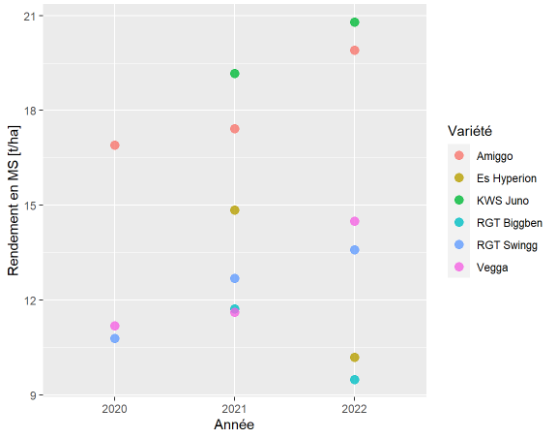
\includegraphics[width=0.6\textwidth]{Image/rendement.png}
\caption{Rendement des parties aériennes de plant de sorgho en fonction de l'année et de la variété}
\label{fig:rendement}
\end{figure}

Ce type de donnée peut être modélisé à l'aide du modèle à deux facteurs catégoriels et une réponse quantitative (ANOVA2) suivant :
\begin{equation}
    Y_{ijk} = \mu + \alpha_{i} + \beta_{j} + \gamma_{ij} + \epsilon_{ijk}
\end{equation}
avec :
\begin{itemize}
    \item $\mu$ : la moyenne générale
    \item $\alpha_i$ : effet de la variété i 
    \item $\beta_j$ : effet de l'année j
    \item $\gamma_{ij}$ : effet d'interaction entre variétés et année
    \item $\epsilon_{ijk}$ : la fluctuation aléatoire entre l'observation k et la moyenne du traitement. 
\end{itemize}

Malheureusement, n'ayant qu'une seule donnée par traitement, le cas d'un plan sans répétition se présente.
Afin de pouvoir tester les facteurs de variétés et d'années, il est nécessaire de supposer un effet d'interaction nul, or, il semble y en avoir un au vu de la figure \ref{fig:rendement}.
Le modèle serait dès lors largement faussé et ne sera donc pas développé.
On peut toutefois remarquer que les variétés Amiggo et Juno paraissent se démarquer des autres par des rendements relativement plus élevés que les autres.

\subsection{Caractérisation de l'architecture racinaire}

Cette section est dédiée au développement des estimations des cinq paramètres principaux précédemment décrits.
D'autres paramètres de ArchiSimple (EL, dSem, dAdv) sont également détaillés, car ceux-ci occupent une place centrale au vu du fonctionnement du modèle.
Les autres paramètres, provenant d'échantillons ou source comme décrit préalablement, ne seront pas différenciés entre variétés ni détaillés dans ce travail.
Ceux-ci sont, pour la plupart, calculés comme la moyenne observée sur tous les échantillons.
Seul CVDD est estimé comme la relation linéaire entre la valeur absolue des résidus du modèle DIDm et les valeurs estimées par celui-ci.
Les graphes et tableaux développant cette régression linéaire sont disponibles en annexe \ref{an:CVDD}.
Les paramètres n'ayant pas pu être estimés (représenté par le / dans le tableau \ref{tab:archisimple}) sont assignés à des valeurs arbitraires tout en restant cohérents avec l'ordre de grandeur du paramètre en question.

\subsubsection{Dmin : Le diamètre minimal}

La figure \ref{fig:boxplot Dmin} représente les distributions de la latérale la plus fine de chaque racine nodale en fonction de la variété.

\begin{figure}[ht]
\centering
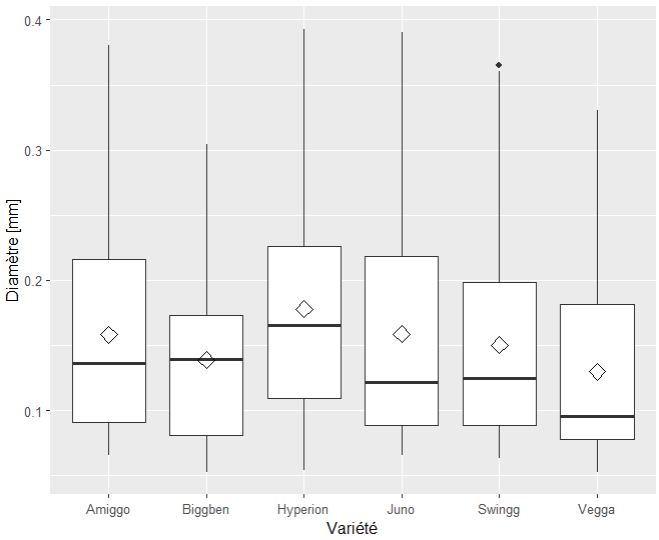
\includegraphics[width=0.5\textwidth]{Image/boxplot Dmin.png}
\caption{Box-plot de la latérale la plus fine pour chaque racine nodale en fonction de la variété}
\label{fig:boxplot Dmin}
\end{figure}

Les distributions semblent visuellement similaires.
Tant les valeurs moyennes et médianes que la largeur des boxplots sont semblables pour chaque variété.
Toutefois, les variétés Biggben, Hyperion et Vegga sont légèrement décalées par rapport aux trois autres.
Le résultat du test ANOVA est qu'au moins une variété a un Dmin significativement différent des autres.
Le tableau de ce test ainsi que la vérification des hypothèses sous-jacentes au modèle sont disponibles en annexe \ref{an:Dmin}.
Le modèle utilisé pour estimer et comparer ces distributions de Dmin est le modèle à un facteur catégoriel fixe suivant :
\begin{equation}
    Y_{ij} = \mu_{A}+\delta_{i}+\epsilon_{ij} \quad \text{avec :} \delta_{i}=\mu_{i}-\mu_{A} \, \text{et} \, \mu_{i} = \text{la moyenne de la variété i}
\end{equation}

Les résultats du modèle sont repris dans la table \ref{tab:summary Dmin} ci-dessous et montrent que seule la variété Vegga, pour laquelle le $\delta_{V}$ est significativement différent de 0 (p-valeur < $\alpha$ = 0.05), a un effet sur le Dmin.

\begin{table}[ht]
    \centering
    \caption{Summary du modèle pour estimer Dmin}
    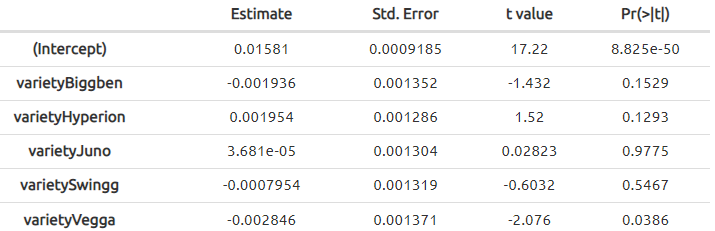
\includegraphics[width=0.75\textwidth]{Image/summary Dmin.png}
    \label{tab:summary Dmin}
\end{table}

La valeur de Dmin retenue pour l'estimation du paramètre Dmin est alors l'estimation du modèle pour la variété Vegga et la moyenne arithmétique des cinq autres variétés pour les autres, soit :

\begin{equation}
    D_{min} = 
    \begin{cases}
        \mu_{V} = \mu_{A}+\delta_{V} = 0.1297 [mm] & \text{pour la variété Vegga} \\
        \frac{\mu_{A}+\mu_{B}+\mu_{H}+\mu_{J}+\mu_{S}}{5}=0.1567 [mm] & \text{pour les autres variétés}
    \end{cases}
\end{equation}

\subsubsection{Dmax : le diamètre maximal}

Les distributions des diamètres de racines nodales en fonction de la variété sont présentées dans la figure \ref{fig:boxplot Dmax}.

\begin{figure}[ht]
\centering
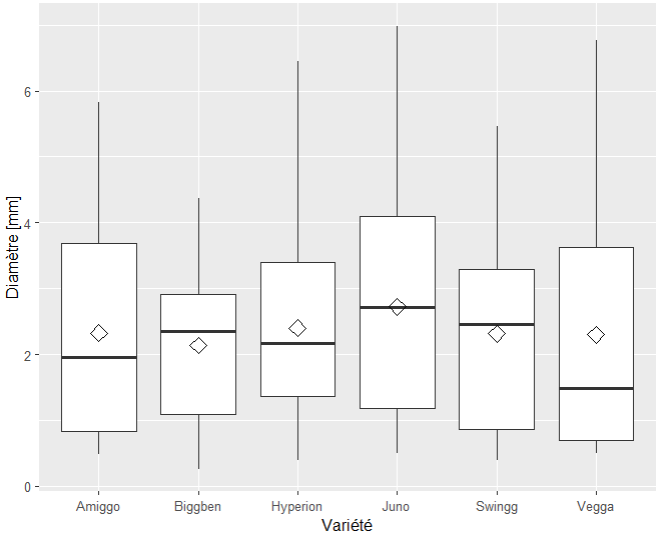
\includegraphics[width=0.5\textwidth]{Image/boxplot Dmax.png}
\caption{Box-plot des diamètres de racines nodales en fonction de la variété}
\label{fig:boxplot Dmax}
\end{figure}
\newpage

Similairement à ce qui a été observé pour Dmin, la distribution des diamètres des racines nodales est fortement similaire pour les six variétés.
Cet aperçu visuel est dans ce cas-ci confirmé par le test ANOVA (table \ref{tab:anova Dmax}) qui confirme l'égalité des distributions de diamètre de racines nodales des différentes variétés (p-valeur > $\alpha$ = 0.05).

\begin{table}[!ht]
    \centering
    \caption{Anova du modèle pour estimer Dmax}
    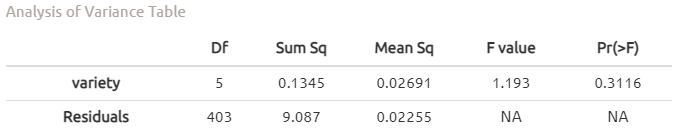
\includegraphics[width=0.75\textwidth]{Image/anova Dmax.png}
    \label{tab:anova Dmax}
\end{table}

L'estimation du paramètre Dmax sera dès lors la même pour les six variétés.
Celui-ci sera alors égal au diamètre maximum observé au sein de tous les échantillons, soit : $D_{max} = 6.984537$ mm.
Le modèle (non signifiatif dans ce cas) est développé en annexe \ref{an:Dmax} ainsi que les tests sur les hypothèses du modèle.

\subsubsection{Drange : la gamme de diamètres}

Les boxplots de Drange pour les six variétés sont présentés figure \ref{fig:boxplot Drange} ci-dessous.
On retrouve, à nouveau, beaucoup de similitudes entre les variétés et le test de variance du modèle (table \ref{tab:anova Drange}) ne laisse pas croire à une différence significative entre les variétés.
Les hypothèses relatives à l'utilisation du modèle sont présentées en annexe \ref{an:Drange}.

\begin{figure}[ht]
\centering
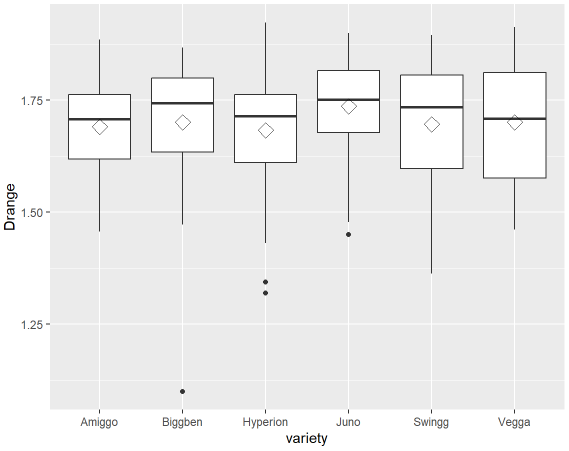
\includegraphics[width=0.5\textwidth]{Image/boxplot Drange.png}
\caption{Box-plot de Drange en fonction de la variété}
\label{fig:boxplot Drange}
\end{figure}

\begin{table}[ht]
    \centering
    \caption{ANOVA du modèle pour estimer Drange}
    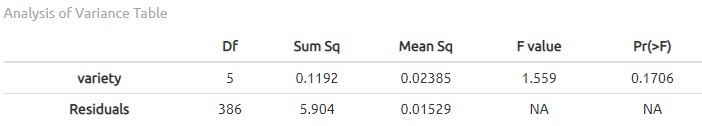
\includegraphics[width=0.75\textwidth]{Image/anova Drange.png}
    \label{tab:anova Drange}
\end{table}

Le résultat du calcul réalisé pour Drange ($2*(D_{max}-D_{min})/(D_{max}+D_{min})$) correspond au coefficient de variation des diamètres.
Ce coefficient permet principalement de comparer la variation au sein de données de moyennes différentes.
Drange n'est pas un paramètre requis en input de ArchiSimple.
L'estimation de celui-ci offre toutefois une vision globale des diamètres des différents systèmes racinaires qui, dans ce cas, seront donc considérés identiques avec un Drange de 1.7011.

\subsubsection{IBD : La distance entre latérales}

Les Boxplots des distances inter-primordium en fonction de la variété est présenté ci-dessous dans la figure \ref{fig:boxplot IBD}.

\begin{figure}[ht]
\centering
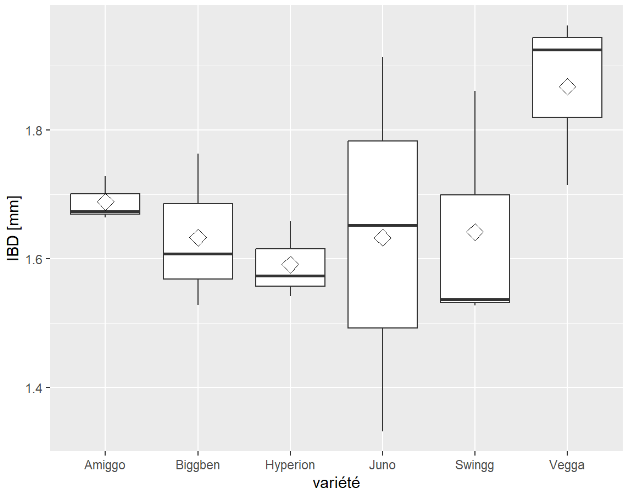
\includegraphics[width=0.5\textwidth]{Image/boxplot IBD.png}
\caption{Box-plot de IBD en fonction de la variété}
\label{fig:boxplot IBD}
\end{figure}

Les distributions, notamment celle pour la variété Vegga sont assez différentes dans ce cas.
Néanmoins, le test ANOVA (table \ref{tab:anova IBD}) n'indique pas de différence significative entre variétés.

\begin{table}[ht]
    \centering
    \caption{Anova du modèle pour estimer IBD}
    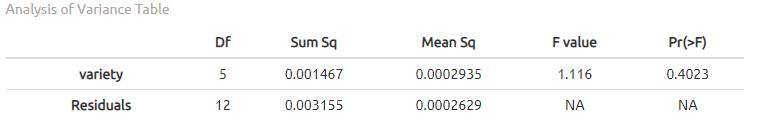
\includegraphics[width=1\textwidth]{Image/anova IBD.png}
    \label{tab:anova IBD}
\end{table}

La figure \ref{fig:inférence IBD} illustre les estimations faites par le modèle ANOVA sur le paramètre IBD.
Celles-ci sont relativement semblables pour toutes les variétés excepté Vegga qui, à nouveau, a une estimation plus élevée.
Des contrastes ont été réalisés afin d'avoir un test statistique plus spécifique à la variété Vegga.
Ces contrastes confirment une fois de plus que les estimations pour les différentes variétés ne peuvent pas être considérées comme étant différentes pour un niveau de confiance de $\alpha = 0.05$.

\begin{figure}[ht]
\centering
\includegraphics[width=0.85\textwidth]{Image/inférence IBD.png}
\caption{Inférence et contrastes Vegga pour IBD}
\label{fig:inférence IBD}
\end{figure}

Dès lors qu'aucun test n'indique un rejet de l'hypothèse d'égalité des moyennes entre variétés, celles-ci auront la même estimation moyenne de distance entre latérales soit : $IBD=1.6761 mm$.

\subsubsection{DIDm : le ratio Dfillle/Dmère}

La figure \ref{fig:plot DIDm} met en relation les diamètres de racines latérales avec le diamètre de leur racine parente par variété ainsi que les régressions linéaires qui en découlent.
Les droites de régressions linéaires semblent à priori significativement différentes pour chaque variété indiquant un effet de la variété, du diamètre de la racine mère et de l'interaction entre les deux sur le diamètre des racines latérales.
La table ANOVA \ref{tab:anova DIDm} confirme que ces effets sont significatifs.
\newpage

\begin{figure}[ht]
\centering
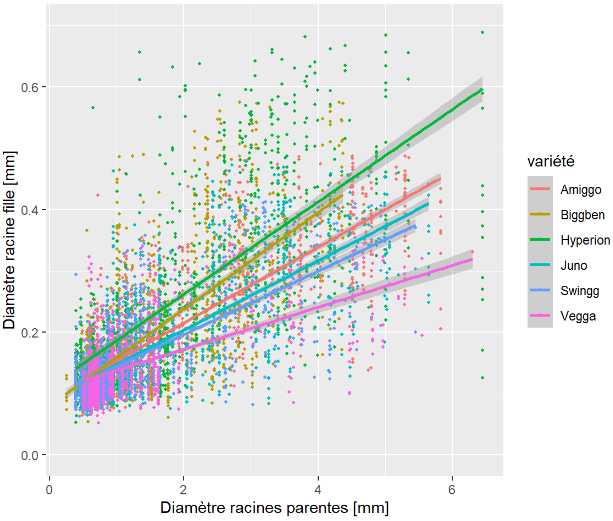
\includegraphics[width=0.6\textwidth]{Image/plot DIDm.png}
\caption{Plot du diamètre des racines fille par rapport à leur racine mère en fonction de la variétés }
\label{fig:plot DIDm}
\end{figure}

\begin{table}[ht]
    \centering
    \caption{Anova du modèle pour estimer DIDm}
    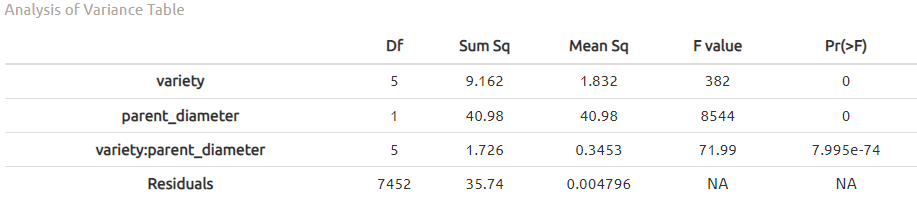
\includegraphics[width=1\textwidth]{Image/anova DIDm.png}
    \label{tab:anova DIDm}
\end{table}

Le modèle linéaire générale utilisé est le suivant : 
\begin{equation}
Y_{ij}=\beta_{0}+\beta_{1}*X_{ij}+\alpha_{i}+\gamma_{i}*X_{ij}+\epsilon_{ij}
\end{equation}
Avec : 
\begin{itemize}
    \item $\beta_{0}$ = l'intercepte de la régression linéaire de Amiggo.
    \item $\beta_{1}$ : effet du diamètre mère sur le diamètre fille pour Amiggo.
    \item $\alpha_{i}$ : effet de la variété sur l'intercepte par rapport à Amiggo.
    \item $\gamma_{i}$ : effet d'interaction diamètre mère et variétés.
    \item $\epsilon_{ij}$ : les résidus du modèle.
\end{itemize}

Les estimations des paramètres du modèle sont présentés dans la table \ref{tab:summary DIDm}.
\newpage

\begin{table}[ht]
    \centering
    \caption{Summary du modèle pour estimer DIDm}
    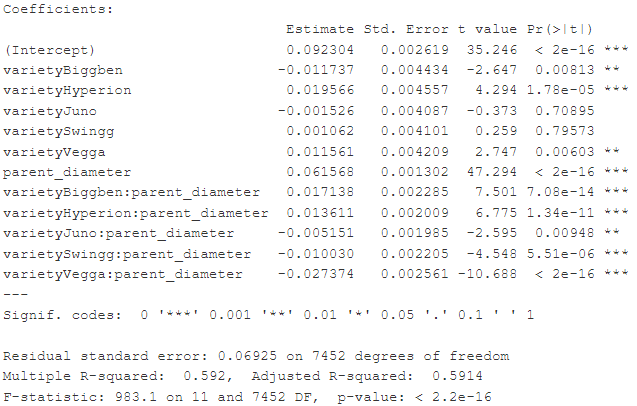
\includegraphics[width=0.68\textwidth]{Image/summary DIDm.png}
    \label{tab:summary DIDm}
\end{table}

Tous les paramètres semblent induire une différence notable dans l'estimation, à l'exception des paramètres des variétés Juno et Swingg.
Cette similitude s'observe sur la figure \ref{fig:plot DIDm} ou les interceptes de ces deux variétés sont très proches.
La même conclusion peut être tirée de l'observation des contrastes en annexe \ref{an:DIDm}.
Les estimations de DIDm qui sera retenue pour le paramètre DIDm sera l'estimation du modèle pour les différentes variétés telles que repris dans la table \ref{tab:emmeans DIDm}

\begin{table}[ht]
    \centering
    \caption{Estimations de DIDm}
    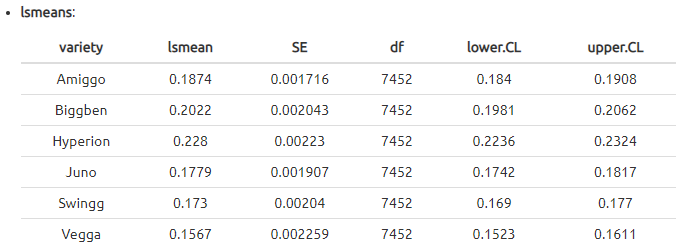
\includegraphics[width=0.6\textwidth]{Image/lsmeans DIDm.png}
    \label{tab:emmeans DIDm}
\end{table}

\subsubsection{EL : l'élongation en fonction du diamètre}

EL correspond à la pente de la relation observée entre le diamètre des racines primaires et leur croissance.
La figure \ref{fig:EL} ci-dessous illustre les données provenant des échantillons en rhizotron ainsi que la régression linéaire estimée par la fonction lm() en R.
\newpage

\begin{figure}[ht]
\centering
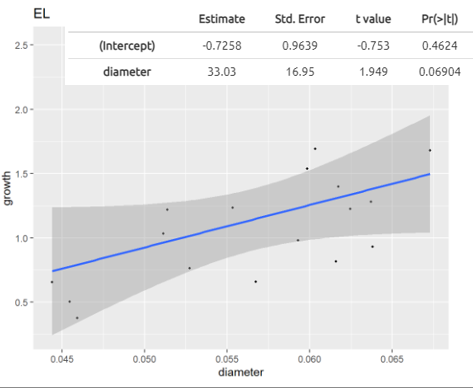
\includegraphics[width=0.55\textwidth]{Image/EL.png}
\caption{Plot et estimation de EL}
\label{fig:EL}
\end{figure}

L'estimation de EL utilisée dans le modèle pour les six variétés de sorgho correspond à la pente de la régression linéaire, soit $EL= 33.03$.
Le choix a été fait de ne pas imposer l'intercepte de cette courbe à passer par l'origine dès lors que le modèle se base sur un Dmin différent de 0 pour définir l'arrêt de la croissance d'une racine.
Par ailleur, cette relation peut également fournir une estimation de diamètre minimum au-delà duquel l'élongation racinaire est arrêtée (Dmin) en suivant le raisonnement suivant :
\begin{equation}
    \begin{cases}
        growth = -0.7258 + 33.03*diameter & \text{Équation de la droite} \\
        Dmin = \frac{0.7258}{33.03} = 0.02197 [cm] = 0.2197 [mm] & \text{Lorsque growth = 0}
    \end{cases}
\end{equation}

Cette estimation de Dmin est nettement supérieure à ce qui a été observé (0.2197 vs 0.1297 et 0.1567) et ne sera dès lors pas retenue pour l'estimation du paramètre Dmin.

\subsubsection{dSem et dAdv : les diamètres relatif de racines séminales et adventives}

Les diamètres relatifs des racines séminale et adventive, respectivement dSem et dAdv dans le modèle, sont mesurés sur base du diamètre maximal Dmax.
dSem est dès lors estimé par le ratio entre la moyenne des diamètres de racines primaires observées et Dmax soit $dSem=\frac{0.5648[mm]}{6.9845[mm]} = 0.08087$
L'estimation de dAdv est quant à elle faite sur base du ratio entre Dmax et la moyenne des diamètres de racines adventive observée, soit $dAdv = \frac{2.3795[mm]}{6.9845[mm]} = 0.3407$
Les deux paramètres sont supposés égaux pour toutes les variétés dès lors qu'il a été observé que les distributions des diamètres de racines primaires et nodales ne pouvaient pas être considérées comme significativement différentes auparavant.

\subsubsection{Tous les paramètres du modèle}

La table \ref{tab:esti.archisimple} reprend les estimations de tous les paramètres d'input du modèle.

\begin{table}[ht]
    \centering
    \caption{Estimation des paramètres de ArchiSimple}
    \includegraphics[width=0.75\textwidth]{Image/paramètre archisimple.png}
    \label{tab:esti.archisimple}
\end{table}

\subsection{Simulation d'architecture de système racinaire}
La durée de simulation a été fixée jusqu'à la fin de la phase végétative, soit environ 40 jours.
\cite{pellerinand_evaluation_1994} observaient que l'extension du système racinaire atteint un maximum quelques jours après la fin de la phase végétative chez le maïs.
Les systèmes racinaires générés par ArchiSimple sont présentés dans la figure \ref{fig:roots} ci-dessous.
\newpage

\begin{figure}[ht]
\centering
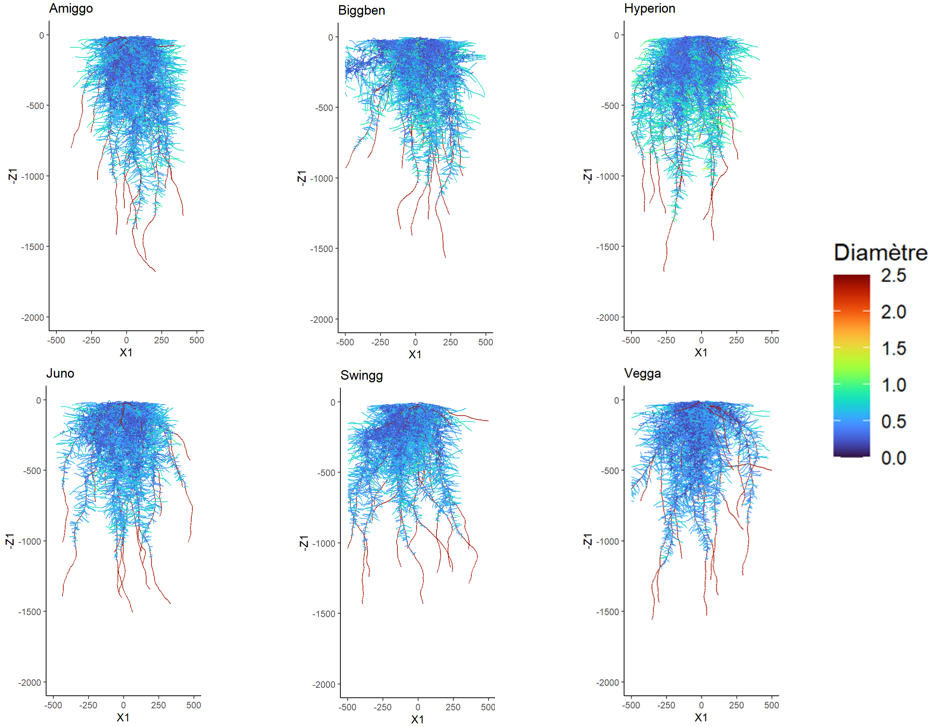
\includegraphics[width=1\textwidth]{Image/roots.png}
\caption{Résultats des modélisations des six variétés}
\label{fig:roots}
\end{figure}

On observe, comme décrit dans la littérature, un système racinaire construit avec des racines adventives de grands diamètres.
Celle-ci s'enfonce profondément dans le sol et donne lieu à des racines latérales qui permettent une meilleure exploration du sol.
Afin de voir comment se construisent ces systèmes racinaires, la figure \ref{fig:roots_day} affiche l'évolution du système racinaire depuis le 10ème jour jusqu'au 40ème par pas de temps de cinq jours pour la variété Amiggo.
\newpage

\begin{figure}[ht]
\centering
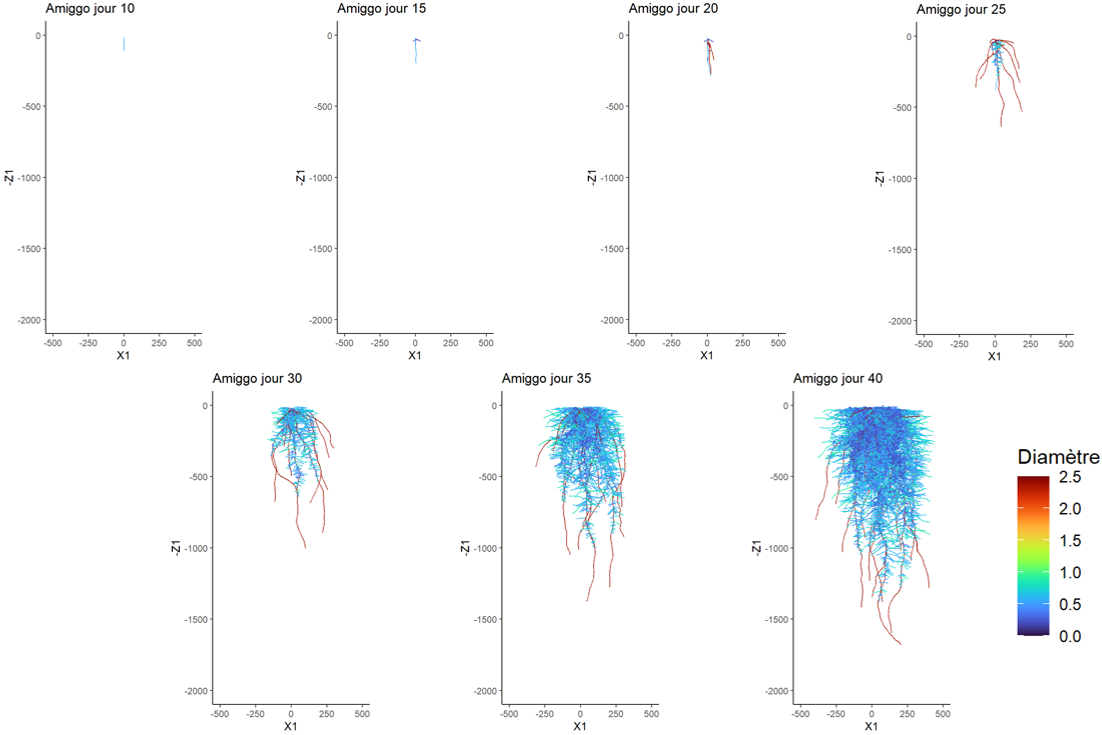
\includegraphics[width=1\textwidth]{Image/root_day.png}
\caption{Évolution de la modélisation tous les cinq jours pour Amiggo}
\label{fig:roots_day}
\end{figure}

Le sorgho ne développe, dans un premier temps, que sa racine primaire.
Au 15ème jour, la racine primaire s'est allongée et on observe un développement de quelques racines latérales sur la racine primaire.
Dès le vingtième jour, les racines nodales commencent à apparaître dans la modélisation.
Au jour 25, la racine primaire est plus ramifiée et certaines racines nodales sont plus longues que la racine primaire.
Après une trentaine de jours, on ne discerne plus la racine primaire, les racines nodales sont encore plus longues et possèdent des ramifications.
Finalement, jusqu'au jour 40, les racines nodales grandissent encore et se ramifient de plus en plus.
Ce développement correspond bien globalement à ce qui pourrait être observé sur un vrai système racinaire de sorgho.

\newpage

\section{Discussions}

\subsection{Commentaire résultats}

\subsubsection{Résultats du modèle pour le sorgho}

Certaine subtilité observable dans la modélisation au cours du temps de la variété Amiggo ne correspondent pas à ce qui a été observé lors des essais en rhizotron.
La racine primaire n'est pas encore observable au jour cinq alors que celle-ci commençait déjà à apparaître dès le troisième jour lors des expériences.
De plus, cette racine primaire comporte assez peu de latérales avant le jour 25 ou celle-ci apparaissent en nombres tandis que les racines observées en développaient davantage aux alentour du 10e jour.
Toutefois, mis à part ces délais dans l'apparition des racines, les modélisations réalisées par ArchiSimple sont en accord avec le développement de réelles racines de sorgho.
\newline

Les résultats pour les six variétés sont relativement similaires, mais cela était attendu au vu des faibles variations d'input précédemment observées sur les échantillons.
Les quelques différences identifiées statistiquement comme étant significative (dmin et RDM) ne semblent donc pas, avec ArchiSimple, engendrer des systèmes racinaires très différents.
Ce résultat est assez complexe à critiquer dès lors qu'aucune étude sur ces systèmes racinaire n'ait encore été réalisée.
Il est cependant remarquable que les résultats de modélisation pour les six variétés de sorgho paraissent être cohérent au niveau de l'ordre de grandeur obtenu pour les profondeurs et l'étendue des systèmes racinaires.
Les valeurs de profondeurs et de largeurs observées dans ces systèmes racinaires fictifs sont reprises dans le tableau \ref{tab:roots}.
Le sorgho étant souvent venté pour avoir des racines pouvant s'étendre jusqu'à deux mètres de profondeur et des racines latérales assez étendues horizontalement, cela conforte en partie la validité des résultats.

\begin{table}[ht]
    \centering
    \caption{Résultats ArchiSimple}
    \begin{tabular}{c|c c c c c c}
    Caractéristique & A & B & H & J & S & V \\
    \hline 
    Profondeur[m] & 1.680 & 1.562 & 1.677 & 1.504 & 1.431 & 1.553 \\
    Largeur[m] & 0.831 & 1.396 & 1.009 & 1.031 & 1.152 & 1.162 \\
    Diamètre moyen [mm] & 0.638 & 0.641 & 0.663 & 0.640 & 0.638 & 0.618
    \end{tabular}
    \label{tab:roots}
\end{table}

Néanmoins, la modélisation manque de réalisme lorsqu'on observe les diamètres de racines nodales.
En effet, toutes les racines adventives qui sont émises ont le même diamètre.
Cela n'a manifestement pas conduit à la formation de système racinaire complètement incohérent lors de ces modélisations.
Malheureusement, au vu du fait que les diamètres sont centraux dans ce modèle par leur implication dans les processus d'élongation (équation \ref{eq:PER}) et de sénescence (équation \ref{eq:LD}), cela affecte fortement la modélisation.
Les répercussions qu'a cette égalité de diamètres entre toutes les racines adventives seront développées plus loin dans ce rapport lors de la discussion sur ArchiSimple.

\subsubsection{Comparaison entre modélisation de Sorgho et de maïs} 

Afin de se faire une idée plus précise des spécificités qu'aurait le système racinaire du sorgho, l'architecture du système racinaire du maïs a également été modélisée.
L'estimation des paramètres a, dans ce cas, entièrement été faite sur base de sources bibliographiques détaillées en annexe \ref{an:Maize}.
Le résultat de cette modélisation est présenté en figure \ref{fig:roots_maize} ci-dessous.

\begin{figure}[ht]
\centering
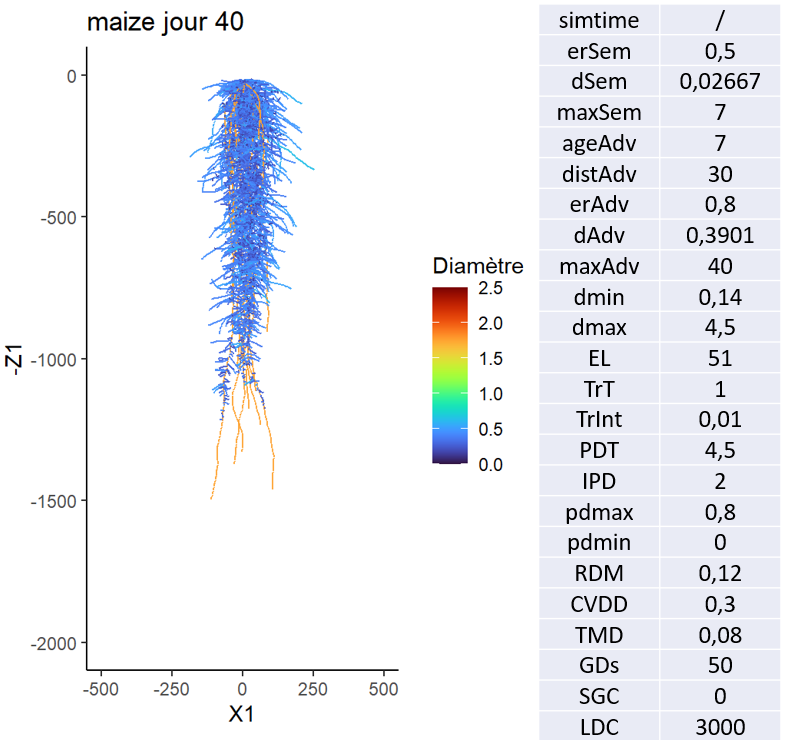
\includegraphics[width=0.6\textwidth]{Image/roots_maize.png}
\caption{Modélisation et paramètres maïs}
\label{fig:roots_maize}
\end{figure}

Le système racinaire alors créer est moins étendu que ceux synthétiser pour le sorgho.
Cette modélisation du maïs donne une profondeur maximale de 1.492 mètres, une largeur de 0.432 mètre et un diamètre moyen de 0.572 mm.
Ces trois valeurs sont chacune plus faibles que celles observées lors des précédentes modélisations de sorgho.
La profondeur atteinte n'est que faiblement inférieure au sorgho, mais les systèmes racinaires produit pour le sorgho couvre une plus grande distance horizontale.
Cette différence vient, d'une part, par des racines adventives qui s'étendent de façon plus verticale chez le maïs et, d'autre part, par les racines latérales qui ont une croissance plus importante chez le sorgho.
\newline

Si on observe bien un système racinaire plus étendu et dense chez le sorgho comme cela est souvent suggéré, il était attendu que les différences de profondeurs soient plus importantes.
Les racines de grands diamètres chez le sorgho devraient, au vu des paramètres observés et des processus du modèle, avoir une élongation bien plus importante que celle du maïs.
Le fait que cela ne soit pas observable peut, en partie être dû à l'estimation de certains paramètres mais il est fortement probable que le fait que les racines adventives sont émises avec le même diamètre engendre en partie ce constat.

\subsubsection{Les échantillons}

Les mesures ayant servi pour estimer les différents paramètres de ArchiSimple proviennent de sources variées.
Certaine sont faites sur des plants de sorgho de fin de culture en champ, d'autre en début de culture en rhizotron et d'autres encore proviennent de sources bibliographiques.
Ces différentes sources vont de pair avec différentes conditions de cultures, différents matériels et différentes méthodes de mesures pouvant influencer les résultats. 
Travailler avec le vivant implique constamment une partie stochastique dans les résultats dû aux éléments imprévisible que conserve les plantes.
Néanmoins, il est possible que les différentes mesures aient été influencés de façon significative par les conditions de culture des plants et les méthodes de mesure.
Cette affirmation est d'autant plus adaptées dans le cadre de ce travail étant donnés que de nombreuses différences sont identifiables dans les conditions de cultures.
En effet, plusieurs différences de traitements sont identifiables entre les échantillons de fin et de début de culture :
\begin{itemize}
    \item Les échantillons en champs ont été confrontées à la compétition, aux aléas climatiques, aux organismes des sols, ... alors que les plants en rhizotron sont maintenus en conditions contrôlées d'humidité, de températures et de lumière.
    \item La présence de champignons au sein des dispositifs en début de culture et l'application du fongicide.
    \item Le milieu dans lequel évolue les racines (perlite vs terre) et les contraintes physiques, biologiques et chimiques qui en découlent.
    \item La nutrition de la plante qui était contrôlée en début de culture et non en champs.
\end{itemize}
Ces nombreux facteurs ont sans aucun doutes affecté le développement de la plante avec une intensité difficilement quantifiable.


\subsubsection{Archisimple }
\citep{pages_modelling_2014-1} (paramètre non exploré par le modèle). \\

ArchiSimple est un modèle plutôt original dans sa façon d'appréhender l'architecture d'un système racinaire.
Les différents processus permettant de faire évoluer le modèle semblent capturer l'essentiel du développement de l'architecture racinaire.
Les inputs requis au fonctionnement du modèle représentent également un atout grâce à leur faible nombre et le fait que ces traits architecturaux sont, pour la plupart, relativement facile à mesurer.
Le fait de ne différencier les racines que part leur diamètre offre une certaine versatilité aux processus qui régissent le modèle, offrant ainsi la possibilité de modéliser presque tout type de système racinaire.
De plus, les différentes relations impliquant les diamètres ont pour la plupart le soutien de différentes études validant son impact sur l'intensité des processus du modèle.
ArchiSimple offre ainsi une approche intéressante, aisée et rapide à la construction d'architecture racinaire.
Cependant, il est apparu dans ce travail que ArchiSimple peut être un peu lacunaire sur certains points.
Celui-ci n'avait pas la prétention de pouvoir remplacer d'autres modèles déjà existants mais plutôt de proposer un modèle versatile qui permet la modélisation de quasiment n'importe quel système racinaire sur la base d'un minimum d'input facilement mesurable.
Les lacunes observées pénalisent principalement la modélisation de système racinaire adventif qui est assez restrictive.
\newline

Tout d'abord, et le plus impactant dans le contexte de ce travail, la façon de définir le diamètre des racines adventives ne correspond pas au développement des Poaceae comme le maïs ou le sorgho.
Ces deux plantes, modélisées précédemment dans ce document, présentent une succession de nœuds qui donne lieu à des racines adventives.
Les échantillons récupérés en champs indiquent que le diamètre des racines nodales émises est alors croissant au fur et à mesure que les nœuds apparaissent.
Or, ArchiSimple ne semble attribuer qu'un unique diamètre aux racines adventives, à savoir $Diametre = dMax*dAdv$.
Cela est particulièrement restrictif dans le cas du maïs et du sorgho ou ces racines représentent, a terme, la totalité du système racinaire.
Cet inconvénient a été contourner en calibrant le paramètre dAdv sur le diamètre moyen des racines adventives.
De cette façon, le système racinaire reste cohérent, mais cela éclipse totalement les variabilités qui seraient observable parmi les diamètres racinaires.
Les premières racines, normalement plus fine, bénéficie de plus de temps pour s'étendre alors que les racines plus jeunes devrait bénéficier d'une vitesse de croissance plus importante au vu de leur diamètre plus important et cela n'est pas du tout pris en compte.
Il résulte alors que des racines avec un diamètre moyen sont émises dès le début développement racinaire et celle-ci atteigne des longueurs trop importantes.
Il serait intéressant d'introduire un paramètre évaluant l'évolution du diamètre des racines adventives en fonction du moment de leurs émissions.
\newline

Ensuite, on retrouve dans ce travail une incohérence entre les paramètres du modèle Dmin et EL.
Ce constat est probablement biaisé par le fait que les échantillons sur lesquels sont calculés EL sont des racines primaires ayant évoluées en rhizotron alors que Dmin provient de racines latérales observées sur des échantillons cultivés en champs.
Néanmoins, les différentes modélisations font face à une dualité entre ces deux valeurs.
Les racines inférieures à 0.2197 mm ne devraient, selon la régression utilisé pour calculer l'élongation potentiel, plus être sujette à une quelconque élongation.
Pourtant, le modèle maintient le processus d'élongation jusqu'au diamètre minimum Dmin qui est bien plus faible (0.1297 ou 0.1567 mm) et qui observerait, selon la régression de EL, une élongation négative.
Cela mène à la conclusion que l'élongation potentielle ne devrait pas être linéaire avec les diamètres.
\newline

En effet, le paramètre EL, considérer comme étant linéaire, n'a pas été observé comme tel par \cite{pellerinand_evaluation_1994}.
Dans le cas présent (et probablement courant) ou celui-ci est estimé sur base de racine de diamètre assez faible, cela pousse la relation du processus d'élongation $PER = EL*D$ (simplification de l'équation \ref{eq:PER}) a estimés une élongation potentielle bien trop importante pour les racines avec des diamètres plus importants.
En outre, la croissance devrait ralentir avec l'âge et la profondeur de la racine tel qu'observer par \cite{pellerinand_evaluation_1994}.
Plusieurs hypothèses justifie cette diminution de l'élongation racinaire.
Cela pourrait provenir du fait que de moins en moins de carbohydrates sont acheminés au plus on s'éloigne des parties aériennes, ou encore des conditions physiques et chimiques rencontrée plus en profondeur.
\newline

Il y a également un problème dans la durée de croissance.
Des simulations de 60 jours engendrent des systèmes racinaire qui s'étendent à plus de trois mètres ce qui est largement supérieur à ce qui serait observé en réalité.
Le paramètre GDs est trop élevé dans notre cas tant pour le sorgho que le maïs.
Ce paramètre mériterait donc d'être estimer à nouveau afin pouvoir limiter la croissance racinaire.
\cite{cahn_relationship_1989} identifie par ailleurs une durée de croissance (GD) différente pour les racines latérales qui ne pourrait pas s'expliquer sur la seule base de leurs diamètres comparé aux autres racines.
\newline

Finalement, une question s'est posée à plusieurs reprises au cours de ce travail de la possibilité de travaillé à l'aide de °Jour comme échelle de temps.
Cette échelle de temps est déjà largement utilisée pour caractériser la croissance aérienne des plantes et son utilisation pour induire l'évolution du système racinaire permettrait la prise en compte de l'environnement de la plante ainsi que ses besoins propres en températures pour se développer.
Plusieurs études lient le développement racinaire au développement aérien, lui-même souvent quantifier en °Jour ce qui a parfois pu complexifier l'estimation des paramètres.
\cite{pellerinand_evaluation_1994} a pareillement identifié un lien entre les températures et le développement du système racinaire.

\subsection{Commentaire sur le sorgho}

Si les printemps secs et les étés déficitaires en eau incitent aux cultures de sorgho, il est encore prématuré de considérer le sorgho comme un candidat pour de grandes cultures en Belgique.
La sélection variétale ne permet pas à ce jour d'assurer qu'une culture de sorgho arrive à terme sans aucun problème.
En effet, le maïs, qui a l'avantage d'être moins exigeant en températures que le sorgho, conserve des rendements plus intéressant à ce jour dans des régions où l'on peut encore observer des années plus fraiches.
L'amélioration et la sélection végétale, encore susceptible à de nombreux progrès pour le sorgho, pourraient permettre d'élargir la gamme de conditions climatiques adaptées à cette culture.
Néanmoins, les trajectoires climatiques promises actuellement pourraient en faire une alternative incontournable dans les régions ou le maïs souffrirait de manque d'eau.
Il pourrait également s'imposer, à une échelle plus modérée, dans des pays comme la Belgique si ses rendements viennent à concurrencer ceux du maïs tout en étant plus résilient.
\newline

Le sorgho conserve tout de même un intérêt particulier dans la recherche.
Il existe encore certains mécanismes participant à sa résilience, pour le moment hors du commun, qui peuvent être identifiés et analysés.
Ces traits peuvent alors participer à orienter la sélection génétique d'autres cultures dans une optique de résilience en réponses aux changements climatiques.

\subsection{Perspective}

L'architecture du système racinaire n'est qu'une étape dans un pipeline permettant de modéliser et de comprendre l'absorption d'eau racinaire et les flux hydriques au sein des plantes.
Les résultats de ArchiSimple est dès lors conçu pour être utilisé par autre modèle permettant d'ajouter une nouvelle dimension qui influence les flux hydriques.
L'architecture générée pourrait par exemple, conjointement avec, entre autre les conductivités axiale et radiale, servir d'input au modèle MARSHALL pour obtenir l'architecture hydraulique du système racinaire.
Les résultats de modélisation obtenus lors de ce travail ne représentent donc pas une fin en soi, mais bien un pas dans un pipeline.
\newline

Les modélisations présentées dans ce travail sont cohérentes, mais semblent omettre beaucoup de caractéristiques de l'architecture racinaire du sorgho, notamment dans le développement de celle-ci.
Il serait dès lors adéquat d'estimer plus précisément les paramètres qui n'ont pas pu être observés sur les échantillons récupérer.
Ces paramètres demandent d'autres expériences assez variées afin d'estimer ces paramètres plus difficilement observables.
\newline

Pour finir, le modèle lui-même est contraignant pour pouvoir représenter un système racinaire fasciculée construit sur des racines adventives comme le sorgho ou le maïs.
ArchiSimple parais intéressant et est déjà très versatile pour construire bon nombre de systèmes racinaires, mais il est nécessaire d'améliorer le processus d'émissions de racines adventives.
Ce processus occupe une place centrale pour les systèmes racinaires considérés dans ce travail et le fait qu'il ne considère qu'un seul diamètre a des répercussions qui se sont avérées critiques dans le modèle.
Le processus d'émission de racines adventives pourrait être amélioré en permettant une augmentation progressive des diamètres des racines adventive émises.
Cette augmentation pourrait se faire sur base du nombre de racines déjà émises, du diamètre de la racine primaire et de Dmax.
Il serait alors possible d'ajouter une équation similaire à l'équation \ref{eq:adv} sans avoir recours à un input supplémentaire pour le modèle.
\begin{equation}
    \begin{gathered}
        dprim = dmax*dsem \\
        dAdv = dprim + \frac{dmax - dprim}{maxAdv}*nAdv
    \end{gathered}
    \label{eq:adv}
\end{equation}
Avec :
\begin{itemize}
    \item dprim : le diamètre de la racine primaire (i.e. dmax*dsem dans ArchiSimple)
    \item dAdv : le diamètre de la racine adventive émise
    \item nAdv : le nombre de racines déjà émises
\end{itemize}
dAdv serait alors calculé au sein du modèle et ne serait plus nécessaire en input.
La première racine adventive aurait dans ce cas un diamètre proche de celui observé sur la racine primaire et augmenterait linéairement avec le nombre d'adventives déjà émise pour, a terme, atteindre dmax.
Toutefois, cette proposition convient à toutes les espèces si deux conditions sont remplies. 
La première est qu'il faut effectivement observer une augmentation des diamètres de racines adventives.
La seconde est qu'il faut que le diamètre maximal soit observé sur une racine adventive.

\newpage

\section{Conclusion}

Ce travail s'inscrit dans un grand travail de recherche sur les flux hydriques au sein des plantes.
L'intérêt porté à ces flux n'est pas nouveau, mais il reste beaucoup de zone à éclaircir.
Certains processus ont pas encore été suffisamment explorés.
Ces flux sont d'autant plus important aujourd'hui au vu du tournant qu'a commencé à prendre la sélection végétale pour inclure la résilience des plantes pour considérer une culture.
\newline

La recherche sur les racines a connu un intérêt plus tardif que pour les parties aériennes de par la difficulté que représente l'échantillonnage de celle-ci.
Beaucoup de processus majeurs sont désormais bien compris et décrit, mais le système racinaire et son influence sur les flux hydriques manque encore quelque peu de précision.
Le système racinaire nécessite, non seulement de prendre en compte beaucoup d'aspect, mais également d'articuler tous ces éléments ensemble pour parvenir à un résultat final le plus précis possible.
\newline

Le sorgho, longtemps cultivés dans des régions semi-arides, pourrait s'imposer dans de nouvelles régions suite aux dérèglements climatiques.
Cette céréale possède de nombreux atouts face aux maïs, notamment des besoins hydriques sensiblement plus faibles, et offre également une multitude de débouchés.
Cette importante résilience hydrique représente un intérêt majeurs face au dérèglement climatique et la question se pose de la contribution du système racinaire dans cette tolérance à la sécheresse.
\newline

Le CIPF a, suite aux nombreux avantages qu'a le sorgho, commencé à prêter attention à cette céréale pour identifier et partager les nombreuses opportunités qu'elle peut apporter dans les régions comme la Belgique.
Des vitrines de tests de cultures de différentes variétés de sorgho sont ainsi réalisés en Belgique par le CIPF depuis 2013.
Les systèmes racinaires échantillonnés lors de ce travail proviennent de six variétés de Sorgho fourrager testées depuis au moins trois ans au CIPF : Amiggo; RGT Biggben; ES Hyperion; KWS Juno ; RGT Swingg et Vegga.
Afin de pouvoir observer au maximum les systèmes racinaires de ces variétés, des premiers échantillons racinaires ont été récupérés en champs après récolte et d'autres ont été réalisés en rhizotron pour en observer la croissance.
\newline

La première étape a été de quantifier des caractéristiques racinaires chez les six variétés de sorgho.
Cinq paramètres racinaires (Dmin, Dmax, Drange, DIDm et IBD) identifier par \cite{pages_seeking_2018} comme capturant assez bien l'entièreté d'un système racinaire ont été retenus pour caractériser les variétés de sorgho observées.
Ces paramètres ont donc été quantifier et les différences ou similitude entre variétés ont été identifiées à l'aide de tests statistiques.
Il en est sorti que les six variétés était, vis-à-vis de ces cinq paramètres, plutôt similaires.
Seuls le Dmin de Vegga et les six DIDm se sont avérés être statistiquement différents parmi les variétés.
\newline

Le modèle utilisé dans ce travail pour modéliser l'architecture des systèmes racinaires est ArchiSimple.
Ce modèle fonctionne sur base de cinq principaux processus : émission, élongation, ramification, croissance radiale et abscission.
Pour fonctionner, ces processus utilise une vingtaine de paramètres demandés en input du modèle.
Le faible nombre d'inputs est un atout de ArchiSimple et est permis par le fait que l'intensité des processus est souvent basé sur les diamètres racinaires.
Cette approche utilisant les diamètres est exclusive à ArchiSimple et assez intéressante dès lors que toutes les relations impliquant le diamètre dans le modèle ont été prouvés comme évoluant avec le diamètre
\newline

Les systèmes racinaires obtenus via ArchiSimple étaient assez semblables pour les six variétés.
Ce résultat est cohérent au vu des faibles variations observées parmi les paramètres fournit en input du modèle.
L'architecture racinaire du maïs a également été générée à l'aide du modèle afin de pouvoir comparer les résultats obtenus pour le sorgho à ceux du maïs.
Il est alors apparu que les architectures générées pour le sorgho occupaient un plus grand volume de sol de par la longueur des racines latérales et les directions, moins verticales, dans lesquelles les racines adventives se développaient.
Cela va dans le sens de nombreux articles indiquant que le sorgho jouit d'un système racinaire puissant qui couvrent plus de volume de sol que le maïs avec des racines pouvant atteindre jusqu'à deux mètres de profondeur.
\newline

Il est apparu que, bien que les systèmes racinaires générés n'étaient pas démesurés, ArchiSimple manque de réalisme dans sa construction de système racinaire adventif.
Les racines adventives, toutes émises avec le même diamètre, limitent la justesse que pourrait avoir ArchiSimple dans la modélisation de certains systèmes racinaires et particulièrement ceux du sorgho.
Les racines adventives devraient observer une augmentation de diamètres au fur et à mesure de leurs apparitions et cela n'est pas pris en compte par ArchiSimple.
Les diamètres étant au centre de beaucoup de dynamiques dans le modèle, cela engendre différents problèmes dans les systèmes racinaires obtenus.
Le paramètre EL, liant le diamètre à l'élongation racinaire, présente également le désavantage d'être constant alors qu'il a été montré que l'élongation racinaire n'est pas linéaire avec le diamètre et est sujette à une diminution avec le temps et la profondeur.
ArchiSimple est donc, bien que très prometteur pour la modélisation d'architecture de système racinaire, parfois un peu lacunaire et mériterait certaines améliorations.
\newline

Finalement, le sorgho ne présente pas encore le profil d'un candidat aux grandes cultures belges.
Les printemps peuvent encore être déficitaire en température pour cette culture et les rendements actuels égalent difficilement ceux de son homologue le maïs.
Néanmoins, il convient de continuer à s'y intéresser tant comme sujet de recherche que comme alternative de culture pour le futur.
Le sorgho représente aujourd'hui un exemple de résilience hydrique et identifier toutes ses particularités peut mener à l'amélioration d'autres cultures en leur inculquant les traits d'intérêts à la résistance aux stress hydriques.
La sélection de sorgho est également encore sujette à de nombreuses avancées en termes de rendements puisque celle-ci est loin d'être aboutie pour nos régions.
Le sorgho pourrait alors bien, à terme, venir à égaler les rendements du maïs tout en conservant une meilleure résilience, ce qui rendrait cette culture incontournable dans de plus en plus de régions du monde. 
\newpage
\thispagestyle{empty} % Supprime les numéros de page et l'en-tête de cette page
\mbox{} % Ajoute un espace vide pour remplir la page blanche
\newpage

\printbibliography
\newpage

% Pour commencer les annexes
\appendix
\pagenumbering{Roman}

\section*{Table des annexe}
\addcontentsline{toc}{section}{Annexe}

% Pour créer une table des matières des annexes
\newcommand{\listappendicesname}{}
\newlistof{appendices}{apc}{\listappendicesname}
\newcommand{\appendices}[1]{\addcontentsline{apc}{appendices}{#1}}
\newcommand{\newappendix}[1]{\section{#1}\appendices{#1}}
\parindent0mm

\listofappendices
\addtocontents{toc}{\protect\setcounter{tocdepth}{-1}} %Pour pas afficher les annexe dans la table des matières principales
\newpage
\thispagestyle{empty} % Supprime les numéros de page et l'en-tête de cette page
\mbox{} % Ajoute un espace vide pour remplir la page blanche
\newpage

\newappendix{Connecting the dots, réseau complet}
\label{an:modelling_full}
\begin{figure}[ht]
\centering
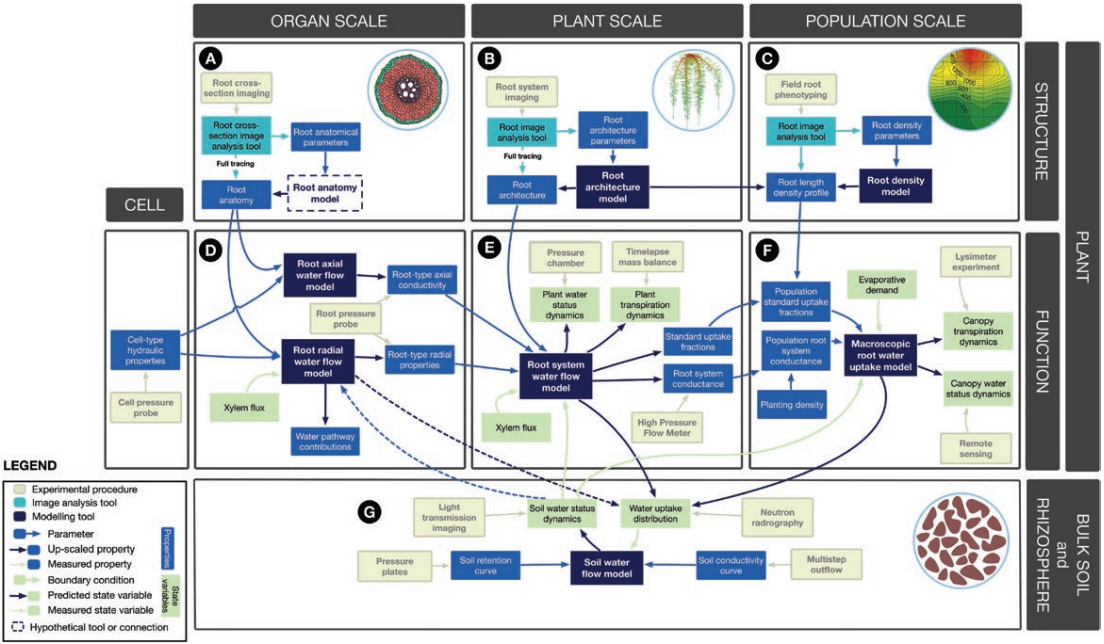
\includegraphics[width=1\textwidth]{Image/modelling.png}
\caption{Réseau complet de \cite{passot_connecting_2018}}
\end{figure}

\newpage

\newappendix{Configuration du scanner}
\label{an:config}
\begin{figure}[ht]
\centering
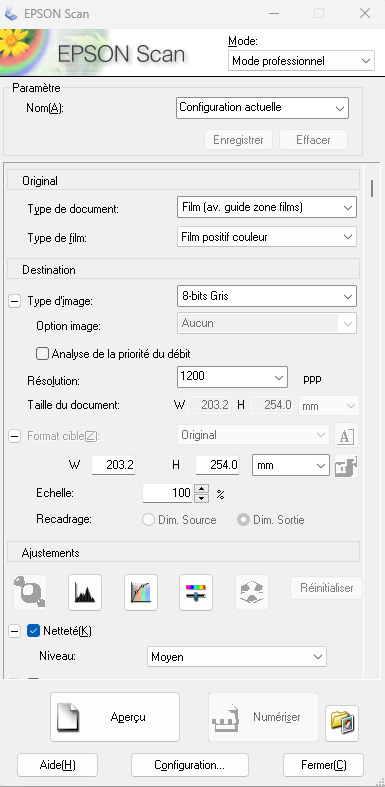
\includegraphics[width=0.5\textwidth]{Image/config scanner.png}
\caption{Configuration utilisée pour numériser les échantillons racinaire}
\end{figure}

\newpage

\newappendix{Protocole des tests de culture du CIPF}
\label{an:protocole_CIPF}
\begin{figure}[ht]
\centering
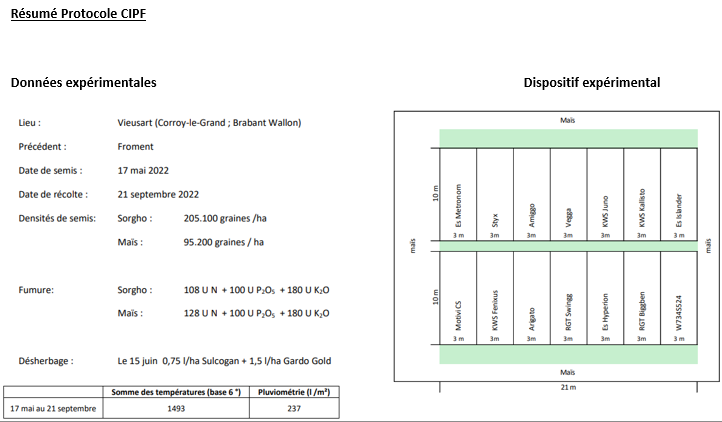
\includegraphics[width=1\textwidth]{Image/protocole CIPF.png}
\caption{Protocole de culture suivi par le CIPF en 2022 \citep{cipf_resultats_2022}}
\end{figure}

\newpage

\newappendix{Solution nutritive de Hoagland}
\label{an:Hoagland}
\begin{table}[ht]
\centering
\caption{Composition de la solution nutritive de Hoagland}
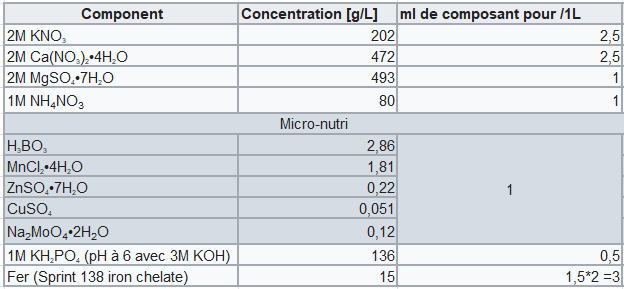
\includegraphics[width=1\textwidth]{Image/hoagland.png}
\end{table}

\newpage

\newappendix{Exemple de tracé de rhizotron}
\label{an:trace}
\begin{figure}[ht]
\centering
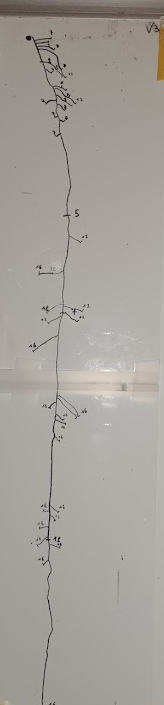
\includegraphics[width=0.235\textwidth]{Image/trace.png}
\caption{Exemple de tracé de rhizotron}
\end{figure}

\newpage

\newappendix{Représentation visuelle d'un fichier RSML}
\label{an:RSML}
\begin{figure}[ht]
\centering
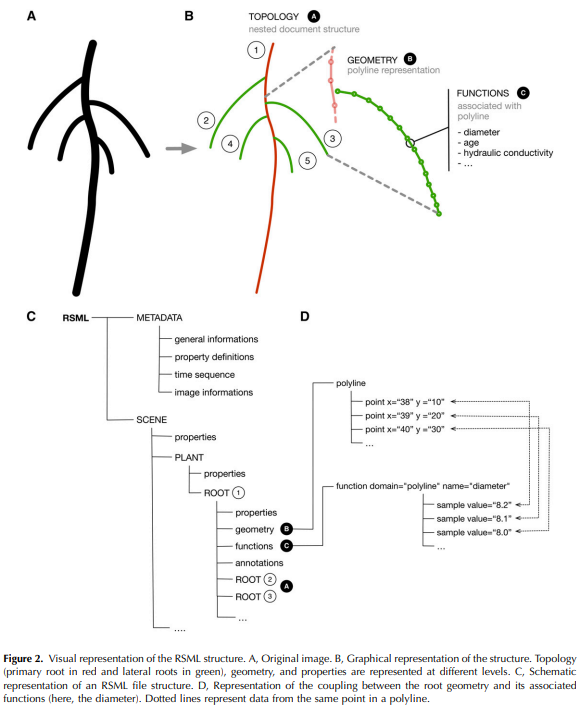
\includegraphics[width=0.8\textwidth]{Image/RSML.png}
\caption{Représentation visuelle d'un fichier RSML provenant de \cite{lobet_root_2015}}
\end{figure}

\newpage

\newappendix{Diagramme ombrothermique culture de Sorgho 2020,2021 et 2022}
\label{an:aerial}
\begin{figure}[ht]
\centering
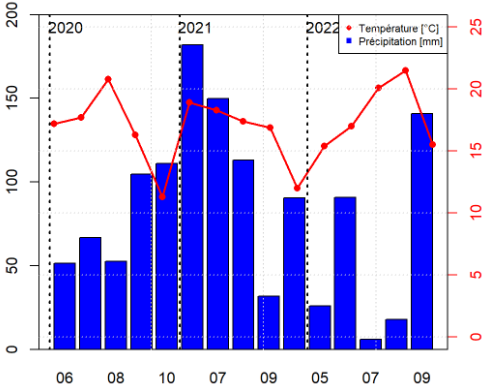
\includegraphics[width=0.8\textwidth]{Image/ombrothermique.png}
\caption{Diagramme ombrothermique des périodes de cultures de sorgho du CIPF}
\end{figure}

\newpage

\newappendix{Estimation monocot}
\label{an:Poaceae}
\begin{figure}[ht]
\centering
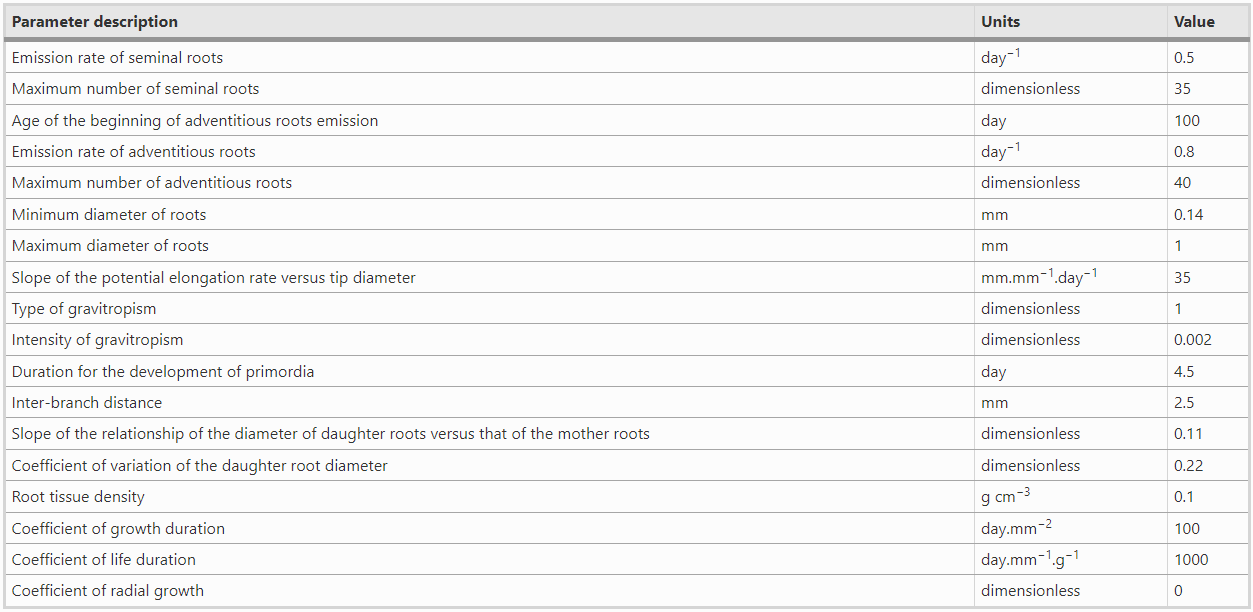
\includegraphics[width=1\textwidth]{Image/parametre Poaceae.png}
\caption{Tableau estimation des paramètres ArchiSimple pour les monocot de \cite{gerard_modelling_2017}}
\end{figure}

\newpage

\newappendix{Dmin}
\label{an:Dmin}
\begin{table}[ht]
\centering
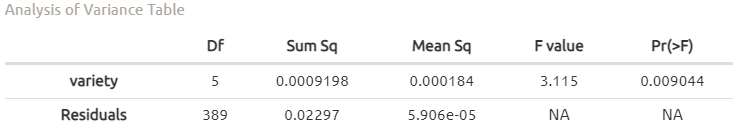
\includegraphics[width=0.65\textwidth]{Image/anova Dmin.png}
\caption{ANOVA du modèle pour estimer Dmin}
\end{table}
\begin{figure}[ht]
\centering
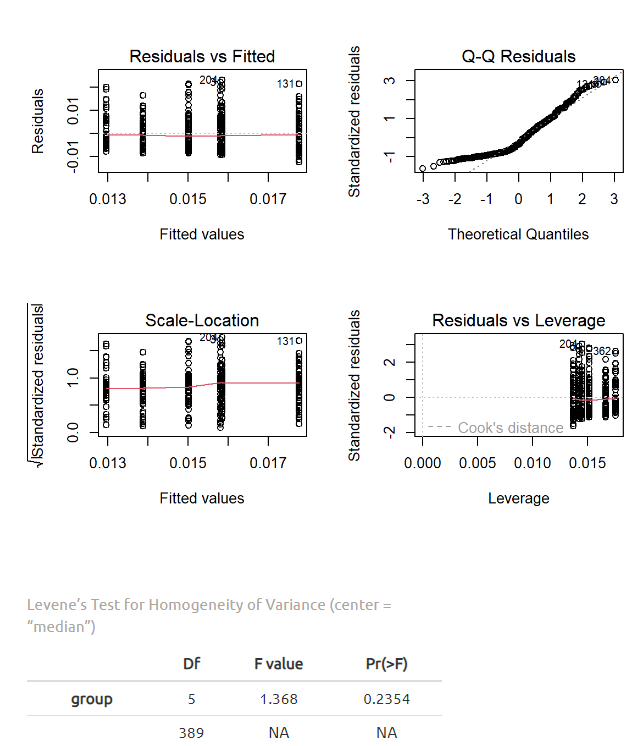
\includegraphics[width=0.65\textwidth]{Image/hypothese Dmin.png}
\caption{Hypothèses Dmin}
\end{figure}
\noindent Indépendance : Assurée par le design et le bon contrôle des conditions expérimentales \\
Normalité : Q-Q plot est OK \\
Egalité des variance : Test de Levene est bon

\newpage

\newappendix{Dmax}
\label{an:Dmax}
\begin{table}[ht]
\centering
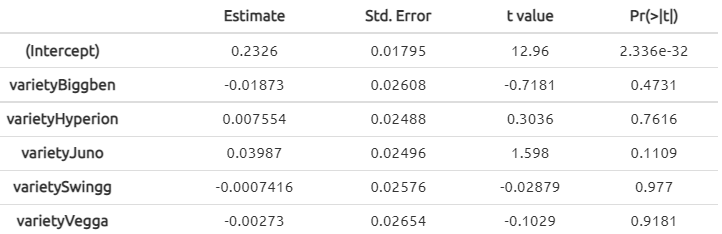
\includegraphics[width=0.6\textwidth]{Image/summary Dmax.png}
\caption{Summary du modèle pour estimer Dmax}
\end{table}
\begin{figure}[ht]
\centering
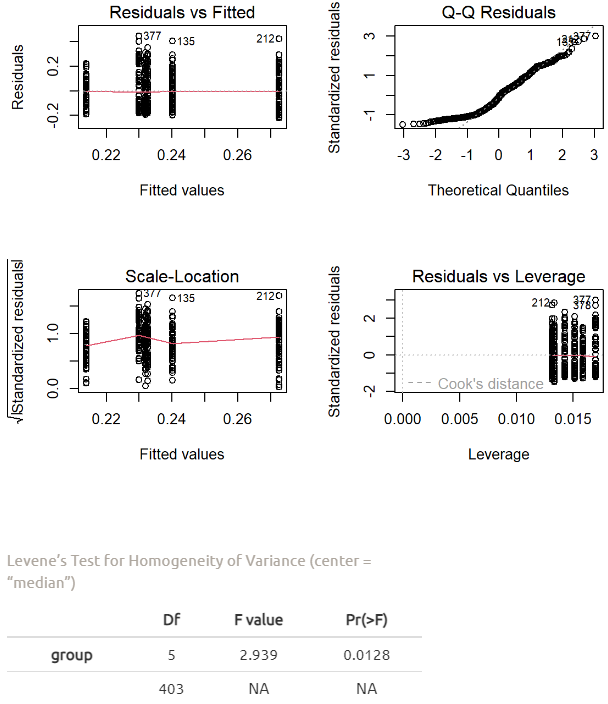
\includegraphics[width=0.6\textwidth]{Image/hypothese Dmax.png}
\caption{Hypothèses Dmax}
\end{figure}
\noindent Indépendance : Assurée par le design et le bon contrôle des conditions expérimentales \\
Normalité : Q-Q plot est OK \\
Egalité des variance : Test de Levene pas bon !

\newpage

\newappendix{Drange}
\label{an:Drange}
\begin{figure}[ht]
\centering
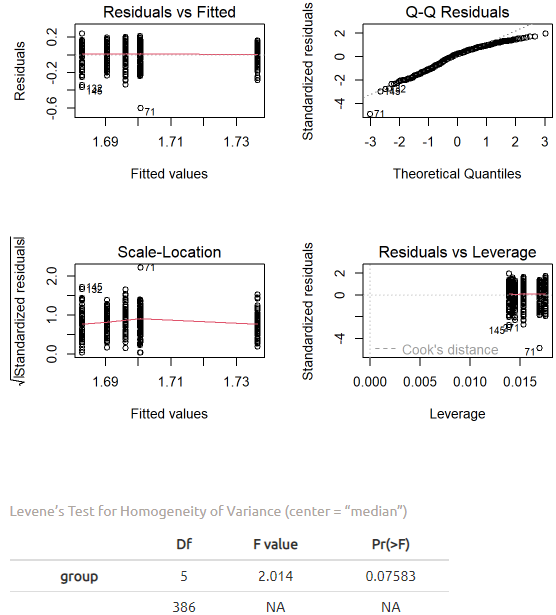
\includegraphics[width=0.6\textwidth]{Image/hypothese Drange.png}
\caption{Hypothèses Drange}
\end{figure}
\noindent Indépendance : Assurée par le design et le bon contrôle des conditions expérimentales \\
Normalité : Q-Q plot est OK \\
Egalité des variance : Test de Levene juste OK !

\newpage

\newappendix{IBD}
\label{an:IBD}
\begin{figure}[ht]
\centering
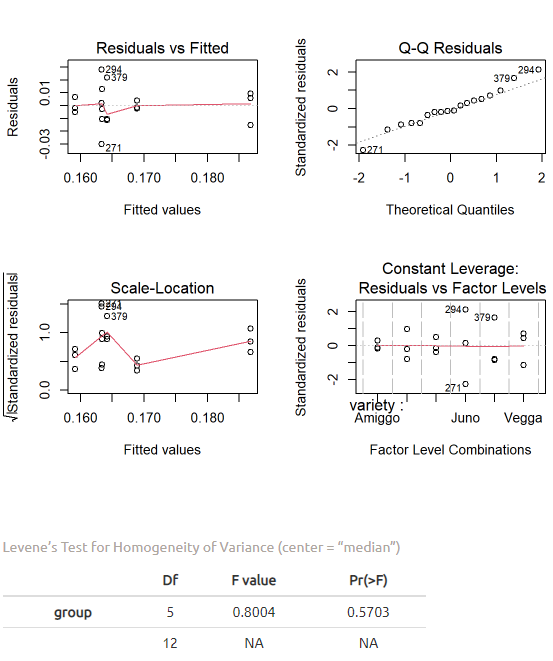
\includegraphics[width=0.4\textwidth]{Image/hypothese IBD}
\caption{Hypothèses IBD}
\end{figure}
\noindent Indépendance : Assurée par le design et le bon contrôle des conditions expérimentales \\
Normalité : Q-Q plot est OK \\
Egalité des variance : Test de Levene juste OK !
\begin{table}[ht]
\centering
\caption{Contrast IBD}
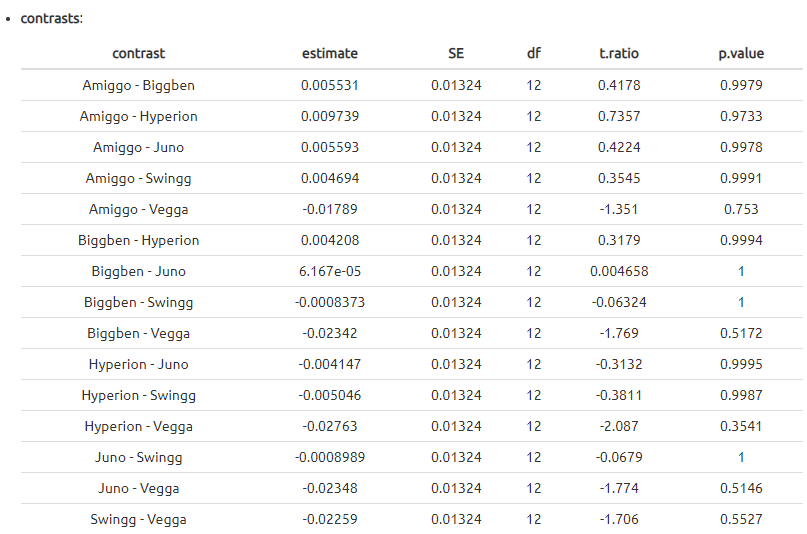
\includegraphics[width=0.5\textwidth]{Image/contrast IBD.png}
\end{table}

\newpage

\newappendix{DIDm}
\label{an:DIDm}
\begin{figure}[ht]
\centering
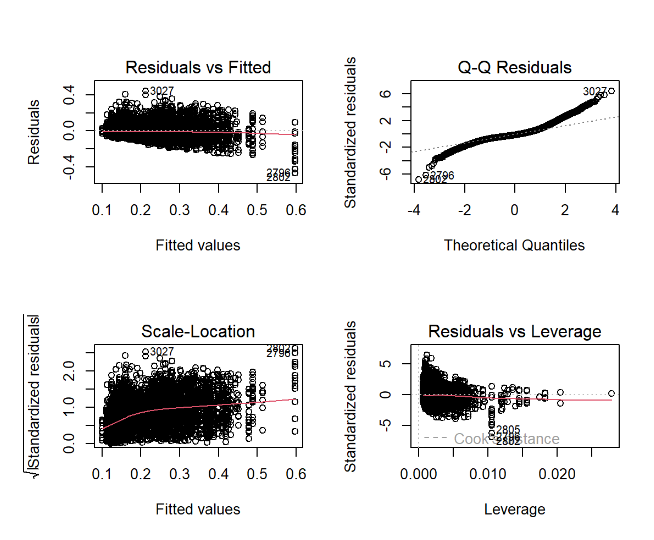
\includegraphics[width=0.6\textwidth]{Image/hypothese DIDm.png}
\caption{Hypothèses DIDm}
\end{figure}
\begin{table}[ht]
\centering
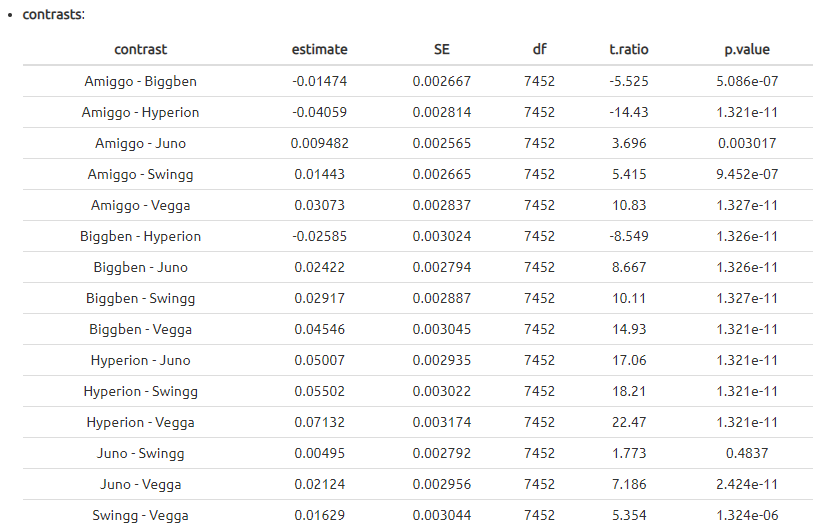
\includegraphics[width=0.6\textwidth]{Image/contrast DIDm.png}
\caption{Contrastes DIDm}
\end{table}

\newpage

\newappendix{CVDD}
\label{an:CVDD}
\begin{figure}[ht]
\centering
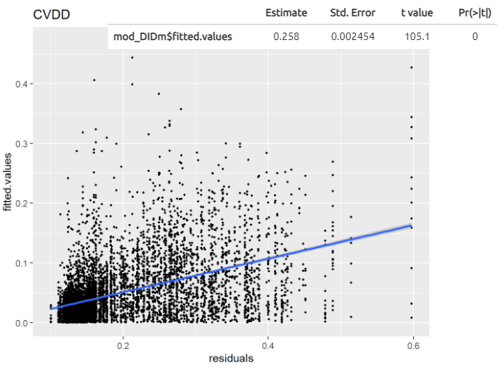
\includegraphics[width=0.55\textwidth]{Image/CVDD.png}
\caption{Graphe et estimation CVDD}
\end{figure}

\newpage

\newappendix{Paramètre maïs}
\label{an:Maize}
\begin{table}[ht]
    \centering
    \caption{Estimation et source des paramètres ArchiSimple pour le maïs}
    \begin{tabular}{c c c}
        Paramètre & Esti & Source \\
        \hline
       simtime & / & / \\
       erSem & 0.5 & \cite{kumar_goyal_how_2021} \\
       dSem & 0.1 & / \cite{pace_analysis_2014} \\
       maxSem & 7 & \cite{kumar_goyal_how_2021} \\
       ageAdv & 7 & \cite{kumar_goyal_how_2021} \\
       distAdv & 30 & / \\
       erAdv & 0.9 & \cite{pages_calibration_2014} adapté \\
       dAdv & 0.3901 & \cite{noauthor_global_2023} \\
       maxAdv & 40 & \cite{pages_calibration_2014} \\
       dmin & 0.14 & \cite{pages_calibration_2014} \\
       dmax & 4.5 & \cite{vanhees_root_2020} \\
       EL & 32.5 & \cite{cahn_relationship_1989} \\
       TrT & 1 & \cite{pages_calibration_2014} \\
       TrInt & 0.01 & \cite{pages_calibration_2014} \\
       PDT & 4.5 & \cite{gerard_modelling_2017} \\
       IPD & 2 & \cite{pages_calibration_2014} \\
       pdmax & 0.8 & / \\
       pdmin & 0 & / \\
       RDM & 0.12 & \cite{pages_calibration_2014} \\
       CVDD & 0.3 & \cite{pages_calibration_2014} \\
       TMD & 0.08 & \cite{pages_calibration_2014} \\
       GDs & 50 & \cite{pages_calibration_2014} \\
       SGC & 0 & \cite{pages_calibration_2014} \\
       LDC & 3000 & \cite{pages_calibration_2014}
    \end{tabular}
\end{table}

\newpage

\newappendix{Diamètre en fonction du noeuds}
\label{an:node_dia}
\begin{figure}[ht]
\centering
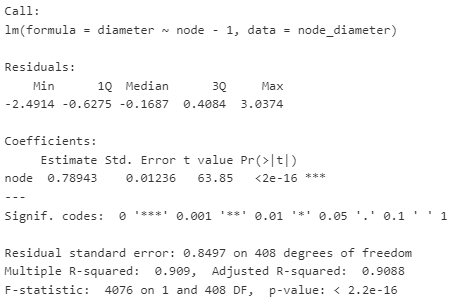
\includegraphics[width=0.7\textwidth]{Image/summary node_dia.png}
\caption{Summary du modèle pour les diamètres en fonction du noeud}
\end{figure}

\end{document}
